En esta parte de la investigación se presentan algunos antecedentes relacionados a la detección y pre-diagnóstico de nódulos en distintos órganos y a través de diversas metodologías. Estos ayudarán a entender el enfoque y obtener bases para un correcto desarrollo del proyecto en cuestión.

\cite{pr_moreira2021deteclung} presenta una investigación relacionada a la elaboración de un sistema CAD (Computer-aided Detection) para la detección y segmentación de nódulos presentes en los pulmones.

Para realizar esta investigación, se tuvo en consideración la realidad que se atraviesa a nivel mundial sobre el cáncer de pulmón, y como este afecta a las personas sin importan su género, convirtiéndolo uno de los tipos de cáncer más mortales según la investigación mencionada. 

La presencia de nuevas formas de detectarlo como el uso de tomografías computarizadas tuvo un gran impacto para la detección temprana de los nódulos en estos órganos, ya que estos pueden significar un futuro desarrollo de cáncer. Sin embargo, realizar un análisis de este tipo de imágenes médicos no era nada trivial debido al complejo proceso de análisis con estas tecnologías. Ante esto, el Deep Learning apareció con una herramienta eficaz para ayudar a los médicos en el análisis de estas imágenes; sin embargo, pese a sus grandes ventajas, su aplicabilidad es muy limitada. Por tal motivo, esta tesis incluye modernos enfoques y técnicas para una detección automática de nódulos pulmonares.

De forma general, el algoritmo presentado en esta investigación consiste en dos bloques. El primero de estos se encarga de la detección de nódulo a través de técnicas de detección de objetos, mientras que el segundo se encarga de la segmentación de este. Los resultados obtenidos fueron del 79\% en recall; sin embargo, esto no fue suficiente para poder considerar al modelo como robusto, por ello, posteriormente, se utilizaron técnicas innovadoras en colaboración expertos en el área. Las anotaciones de los especialistas, junto con los resultados del sistema, mejoraron el desempeño general de la detección.

Para aumentar aún más las capacidades del sistema, se desarrolló en la parte final de la investigación un modelo de Deep Learning para la detección automática y la segmentación de nódulos pulmonares a través de imágenes tomográficas. Este también consistió en dos bloques, uno encargado de la segmentación automática y otro que corrige el anterior en base a dos puntos en los límites del nódulo. El modelo consiguió demostrar su capacidad para corregir la segmentación de nódulos pequeños, además de segmentar los nódulos no sólidos, los cuales presentaban un reto para el sistema.

\cite{pr_felgueiras20193dlungnod} reafirman la importancia de construir este tipo de sistemas mencionando al cáncer de pulmón como el principal tipo de cáncer en causar muertes en todo el mundo.

El sistema desarrollado en esta investigación fue basado en el diagnóstico a través de imágenes tomográficas que comúnmente es realizado por un médico experto; sin embargo, se menciona que este análisis siempre está sujeto a errores ya que existe mucha subjetividad en este tipo de diagnóstico, lo que conlleva muchas veces errores de detección. Además de la existencia de la tendencia al rechazo hacia esto tipo de sistemas CADx (Computer-aided Diagnosis) por parte de los médicos, esto debido a la fata de comprensión del cómo se realiza este tipo de pre-diagnóstico.

Para afrontar esta desconfianza a este tipo de sistemas, se menciona la existencia del Deep Hierarchical Semantic Convolutional Neural Network (HSCNN) que añadía a la capacidad de predecir si un nódulo era maligno o benigno, la función de otorgar evidencia visual del pre-diagnóstico a través de la predicción de las características del nódulo. Sin embargo, el conjunto de datos usado en esta investigación difería de las evaluaciones de los propios médicos. Por tal motivo, en la presente investigación se puso como un objetivo probar si la disminución de esta varianza en los datos podría mejorar los resultados del modelo HSCNN.

A través de un análisis de los datos, se logró mejorar la descripción de características. Este nuevo conjunto de datos fue revisado por especialista para comprobar su validez antes de ser ingresado al modelo HSCNN para predecir si un nódulo era maligno o benigno. Este proceso se hizo a través de un k-folds igual a 4 junto con cross-validation.

Los resultados fueron comparados con el modelo inicial, y se obtuvo que el nuevo HSCNN era mejor solo cuando se trataba de predecir si un nódulo era maligno. Las métricas del nuevo modelo fueron de 0.78 en accuracy, el AUC de la curva ROC es de 0.74, una sensibilidad 0.83 y una especificidad de 0.89, frente a las métricas de modelo original que obtuvo un accuracy de 0.84, un AUC de la curva ROC de 0.86, sensibilidad de 0.71 y una especificidad de 0.89. Esto significó que el modelo se equivocaba más cuando los nódulos a analizar eran pequeños. En general, los resultados distaron de los propios del modelo inicial, esto es debido a la reducción considerable de imágenes del conjunto de datos original. 

\cite{pr_supanta2021desalgdetec} menciona la incidencia de cáncer de pulmón en el Perú en el periodo 2010-2012 con un gran número de 3 121 casos diagnosticados, convirtiéndolo en el tercer tipo de cáncer más común en el país, y ocupa el segundo lugar en mortalidad con un número de 2 591 de muertes en el mismo periodo, esto debido al tardío diagnóstico de este mal. Por este motivo, es obvia la necesidad de realizar un examen de detección temprana donde es posible un tratamiento y, posteriormente, una posible cura a esta enfermedad. 

La investigación presenta una forma de realizar detección de nódulos pulmonares a través de imágenes radiográficas digitales que comúnmente presentan problemas como baja claridad y resaltado de las características, por ende, generan dificultades para realizar un correcto análisis de este tipo de imágenes. Las técnicas usadas son corrección gamma, análisis de proyecciones, erosión, filtros geométricos, dilatación, filtro de convergencia y la umbralización por el método Otsu, esto aplicado a un conjunto de datos de 50 radiografías de tórax.

Los resultamos muestran una sensibilidad del 0.91, especificidad de 0.96 y precisión de 0.94. 

Otra investigación relacionada a detectar alguna enfermedad a través de técnicas de Deep Learning y visión por computadora es la presentada por \cite{pr_monroy2021disvc} donde toma a la enfermedad de Parkinson como mal a detectar, esto a través del análisis de la escritura de una persona. Para tal objetivo, en la investigación se desarrolló un modelo de visión computacional para el pre-diagnóstico de esta enfermedad.

La metodología empieza con la adquisición y preprocesamiento de los datos, para posteriormente usar técnicas de extracción de características como SIFT, SURF, ORB y HOG. Estos serán ingresados a un modelo de Machine Learning (SVM, RF, KNN) que finalmente realizará una clasificación. Además, se usaron diferente arquitectura de Redes Neuronales Convolucionales como Inception, VGG16, VGG19, LeNet y ResNet50.

Los resultados finales fueron un 0.99 en accuracy, 0.99 en precisión, 0.99 en recall, 0.98 en F1-score y AUC.

\cite{pr_kang2022thysegclass} muestran la frecuencia de nódulos tiroideos en los diagnósticos, estando presente en el rango de 19\% y 68\% de todos los casos clínicos recopilados de personas adultas. El cáncer de tiroides es el número 9 en incidencia, mientras que es el número 6 en mortalidad, esto a nivel mundial según datos del 2018.

Se menciona que es importante tener métodos menos invasivos para determinar el cáncer de tiroides, teniendo en cuenta además que es necesario la detección a tiempo, pues esto aumenta la probabilidad de ser curado. El análisis de imágenes de ultrasonido es una buena opción a el análisis de, por ejemplo, cirugías. Sin embargo, esta forma de diagnóstico depende mucho de la experiencia del médico especialista, lo cual vuelve a este tipo de análisis muy subjetivo.

La segmentación y clasificación son herramientas claves dentro de un sistema de diagnóstico asistido, siendo ambos muy relacionados entre sí, pues comparten ciertas características de las imágenes (bordes de las imágenes pueden ser usados para la clasificación y segmentación). Afrontar ambas tareas al mismo tiempo en un solo modelo podría ser más robusto.

La red MTL propuesta en uno de los antecedentes es similar a una red de segmentación multiclases que genera como salida mapa de segmentación y predicciones categóricas.

La investigación presentada en este antecedente se centra también en una red MTL que también realizará procesos de segmentación y clasificación.

La metodología empieza con la data. Esta fue recolectada del West China Hospital. Se tuvieron 4 493 imágenes de ultrasonido, cada uno de un paciente. En específico, 2 576 imágenes pertenecen a nódulos benignos, mientras que 1 917 son malignos. Las anotaciones fueron verificadas por especialistas.

Para la evaluación de la clasificación se usó el accuracy, f1-score, ROC, área bajo la curva ROC (AUC). En el caso de la segmentación, se usó Dice coefficient y Intersection of Union (IoU).

Además, se definieron 3 medidas para cuantificar la inconsistencia al nivel de las tareas. El primero de estos evalúa a la clasificación, el segundo por la tarea de segmentación de segunda clase, y el tercero es para la segmentación de tercera clase.

El modelo construido en esta investigación se basó en MSL (Multi Stage Learning) y MTL (Multi Task Learning). Se diseño una red MS-MTL. Además, se determinó diferentes tipos de consistencia de tareas: intra e inter task consistency.

Los resultados fueron extraídos de 3 modelos CIsNet, MS-MTL y MS-MTL con intra e inter task consistency. La medida AUC obtenida para cada modelo es 0.9277, 0.9523 y 0.9608, respectivamente. Además, se determinó que el intra task cosistency y el MSL aumenta el desempeño de la segmentación. El caso de inter task consistency con MTL mejora el desempeño de las tareas de clasificación y segmentación. Con la combinación de ambas tareas de consistencias también se demuestra su efectividad.

El método usado en esta investigación se muestra en la Figura \ref{2:fig101}.

\begin{figure}[H]
	\begin{center}
		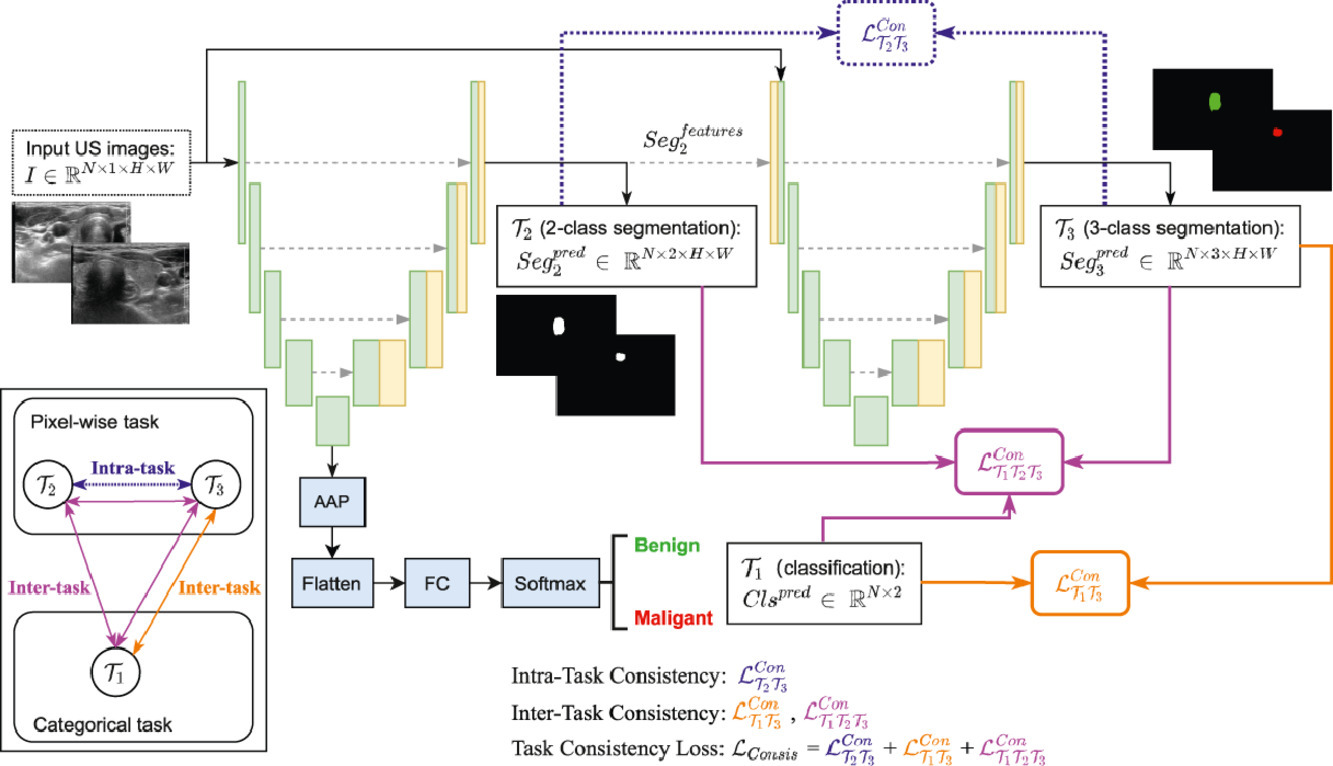
\includegraphics[width=1.00\textwidth]{2/figures/antecedente_4.jpg}
		\caption[Representación del método desarrollado]{Representación del método desarrollado. \\
		Fuente: \cite{pr_kang2022thysegclass}. \textit{Thyroid nodule segmentation and classification in ultrasound images through intra- and inter-task consistent learning}.}
		\label{2:fig101}
	\end{center}
\end{figure}


\cite{pr_sun2023classthynvit} presenta el problema de clasificar nódulos tiroideos nivel 3 debido a pocas características representativas que diferencien a los nódulos benignos de nivel 3 con los nódulos malignos, esto conlleva a obtener bajas precisiones en el pre-diagnóstico. Ante esto, en el artículo se presenta un modelo clasificador de nódulos tiroideos con ViT (Vision-Transformer-based) y el contrast learning. Estas técnicas ayudaron a minimizar la distancia de características en nódulos de una misma clase, lo cual mejora la capacidad predictiva del modelo. Finalmente, en la fase de testeo del modelo se logró un accuracy de 0.869, mientras que las demás métricas indican la superioridad frente a otros modelos clásicos de Deep Learning que también son usados para clasificar.

En la Figura \ref{2:fig102} se presenta la arquitectura de Vison Transformer desarrollada.

\begin{figure}[H]
	\begin{center}
		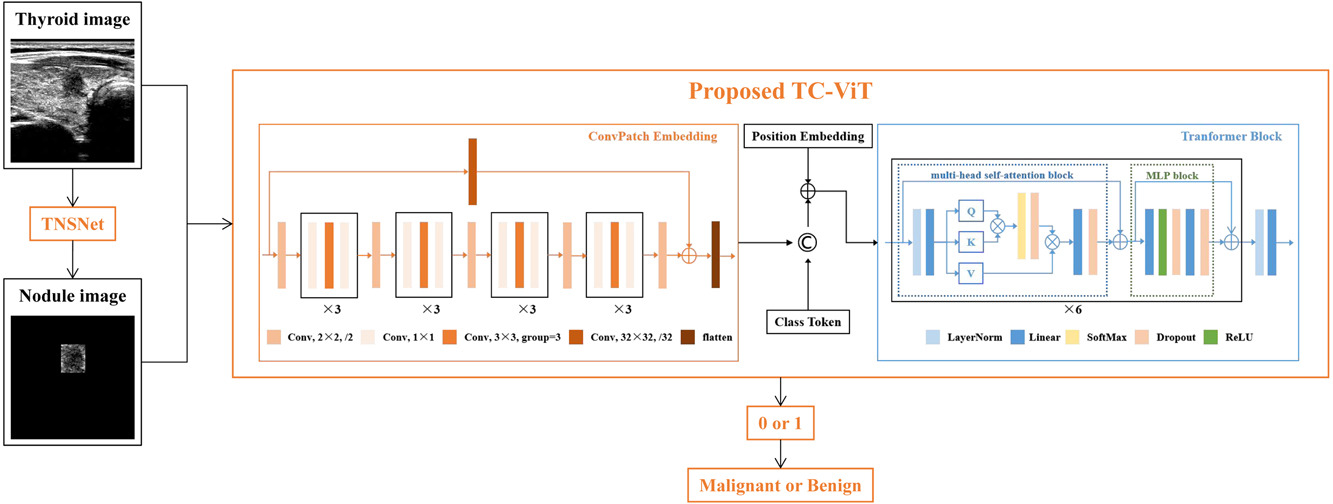
\includegraphics[width=1.00\textwidth]{2/figures/antecedente_5.jpg}
		\caption[Arquitectura de modelo TC-ViT]{Arquitectura de modelo TC-ViT. \\
		Fuente: \cite{pr_sun2023classthynvit}. \textit{Classification for thyroid nodule using ViT with contrastive learning in ultrasound images}.}
		\label{2:fig102}
	\end{center}
\end{figure}


\cite{pr_zhang2023madlap} presenta el nivel de importancia de poseer una buena base de datos etiquetada correctamente para lograr entrenar un buen modelo de Machine Learning. En este artículo se desarrolla y presenta a la herramienta Multistep Automated Data Labelling Procedure (MADLaP) que facilita y automatiza el proceso de etiquetado de datos relacionados a nódulos tiroideos. Este incluye el procesamiento de leguaje natural basado en reglas, el Deep Learning para segmentación de imágenes y el reconocimiento óptico de caracteres. MADLaP fue desarrollado en la fase de entrenamiento con datos de 378 pacientes, mientras que en la fase de prueba se usaron datos de 93. Este obtuvo finalmente un accuracy de 0.83.

\cite{pr_deng2022autclass} ponen al cáncer de tiroides como el que más ha prevalecido en las últimas 3 décadas. Existen diversos sistemas que ayudan a la detección de los nódulos en esta glándula; sin embargo, muchos de estos solo se limitan a determinar si un nódulo es maligno o benigno, y no muestran el porqué de la toma de esa decisión por parte del sistema, lo cual genera desconfianza entre los especialistas al momento de usarlos. Para afrontar esto, se desarrolla primeramente una estratificación de riesgo basada en el léxico estandarizado ACR TI-RADS. Posteriormente, se realiza la clasificación entre benigno y maligno. De formar general, el método realizará una caracterización del nódulo basado en ACR TI-RADS para detectar su nivel de riesgo y la clase al que pertenece (benigno o maligno). Los resultados muestran en la evaluación un accuracy de 0.9355, un sensitivity de 0.9386 y una specificity de 0.9314. 

Se realizó la notación de las imágenes de nódulos con los indicadores del diccionario de ACR TI-RADS. Para afrontar el desbalanceo de la data, se realizó un proceso de mejora de la data creando imágenes a través de giros, recortes y mezclas. Se extrajeron las áreas de interés de las imágenes a través de una red en cascada. Se quitaron las anotaciones manuales en las imágenes (limpieza de imagen). Una vez concluido con el procesamiento de las imágenes, se realizó la construcción y ejecución del modelo de Deep Learning Multi-Task Learning (MLT). Finalmente, el modelo obtenido fue comparado con otros a través de los siguientes indicadores: accuracy, sensitivity, specificity y el área bajo la curva. 

\cite{pr_wang2020autodiag} mencionan que los nódulos tiroideos son uno de los primeros síntomas que podrían conllevar a un cáncer en la tiroides. Este tipo de cáncer es uno de los que tiene mayor incidencia y que esta tendencia ha ido en crecimiento durando los últimos 30 años.

Además, se menciona que, para ayudar a esta detección, se han propuesto anteriormente varios sistemas de diagnóstico asistido; sin embargo, estos solo realizan dicho proceso a través de solo una imagen de ultrasonido en vez de usar todas aquellas que se obtienen de un examen. Por esto, en este artículo, se desarrolla un modelo de Deep Learning para el pre-diagnóstico de tiroides a través de varias imágenes de ultrasonido. Esto a través de una integración de todas las características de las imágenes realizadas en un examen. 

La base de datos usada fue construida, y se obtuvieron resultados perfectamente comparables con los resultados de los antecedentes revisados en este artículo.

La metodología consistía en la construcción de tres redes distintas: feature extraction network, attenntion-based feature aggregation network, classification network. Estas tres redes juntas forman el modelo objetivo desarrollado en este artículo.

En general, la metodología consistía en, primero, la construcción del conjunto de datos que se conforma de imágenes de ultrasonido procedentes de un hospital. Se recolectaron cerca de 7 800 imágenes de 1 046 exámenes de entre los años 2015 y 2018. En segundos lugar, se realizó el etiquetado de los datos. Estas anotaciones se realizaron de acuerdo con los exámenes en general, y no a cada una de las imágenes que la conforman. Luego, se realizó la separación de la data en entrenamiento, prueba y validación. En la parte final de experimentación, se realizó un preprocesamiento con Data Augmentation y se definió 100 épocas para la fase de entrenamiento. El modelo ganador de la fase de validación fue probado con la data de prueba. Las métricas usadas para la evaluación fueron el accuracy, sensitivity (true positive rate) y el área bajo la curva (AUC ROC).

La Figura \ref{2:fig103} muestra la arquitectura propuesta en esta investigación.

\begin{figure}[H]
	\begin{center}
		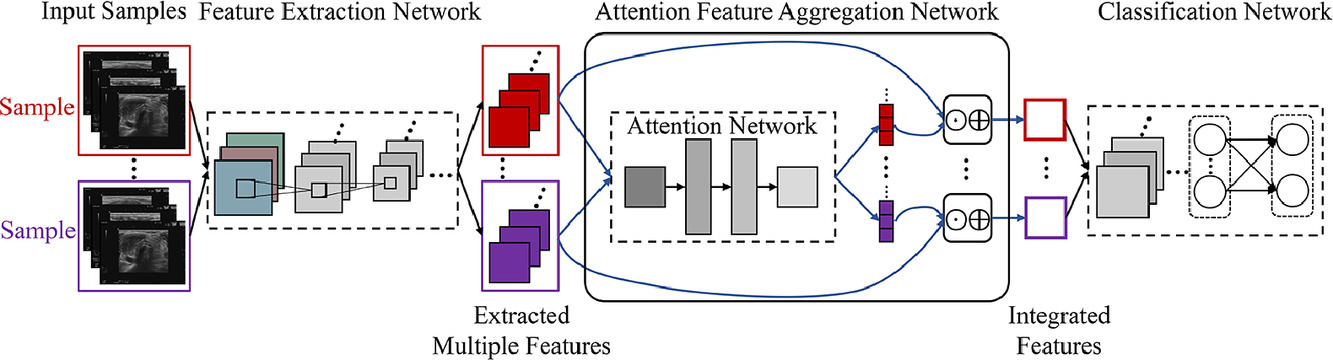
\includegraphics[width=1.00\textwidth]{2/figures/antecedente_8.jpg}
		\caption[Arquitecura de la red desarrollada]{Arquitecura de la red desarrollada. \\
		Fuente: \cite{pr_sun2023classthynvit}. \textit{Automatic diagnosis for thyroid nodules in ultrasound images by deep neural networks}.}
		\label{2:fig103}
	\end{center}
\end{figure}


\cite{pr_sun2022tnsnet} mencionan que, en el sistema endocrino, un problema muy común son los nódulos tiroideos. Normalmente estos pueden ser sólidos o de otras variadas texturas. La incidencia de esta enfermedad se ha ido incrementando a través de los años. Comúnmente se usan las imágenes de ultrasonido para detectar estos nódulos, esto lo hacen en tiempo real, tiene bajo costo y no es invasivo, por cual es una buena opción. Estas imágenes pueden otorgar información valiosa de los nódulos como los márgenes, ecogenicidad, calcificación, composición, etc. Además, existe el Thyroid Image Reporting y el sistema de datos TI-RADS que pueden cuantificar las características otorgadas por las imágenes de ultrasonido y evaluar si es benigno o maligno. Sin embargo, estas imágenes pueden traer problemas como bajo contraste y ruido de moteado, lo cual genera retos para extraer sus características. Este problema puede superarse a través de una correcta segmentación de los nódulos tiroideos. Así, la segmentación es un paso importante para realizar un pre-diagnóstico correcto. Esto puede ser aplicado a la evaluación automática en TI-RADS para facilitar la clasificación de los nódulos. Se añadió un shape-supervised path para mejorar la identificación de la forma, y así lograr una mejor segmentación.

La data que usaron se obtuvo de diversos escáneres disponibles comercialmente, juntando 3 786 imágenes de ultrasonido de nódulos tiroideos. Posteriormente, se realiza un preprocesamiento para estandarizar la data. Se realizó un proceso de limpieza de las imágenes para quitar los datos privados de los pacientes, y borrar imágenes erróneas. Se propuso TNSNet para asegurar una mejor detección y segmentación. Este modelo es un dual-path network que contiene dos partes region path y shape path. Ambos caminos se enfocan en las características de bordes y texturas (cada uno de estos para cada camino).

Se diseñó un dual-path loss function para el entramiento de ambos caminos del modelo. Para el camino de región, se usó el binary cross-entropy loss y el generalized Dice loss, ambos para entrenar la región de segmentación de los nódulos tiroideos. En el caso del segundo camino (camino de la forma) se combinó el Hausdoff distance loss y un modificado active contour loss. Esto fue construido para el entrenamiento del contorno de segmentación.

Las métricas usadas para evaluar la segmentación del modelo son Dice simialrity coefficient (DSC), sensitivity, specificity y el accuracy.

Los resultados muestran que en el caso de los nódulos benignos todos los modelos (el construido en el artículo y los de referencia) logran buenos resultados, esto debido a la buena calidad de las imágenes. En el caso de los nódulos malignos, el modelo TNSNet superó por completo a los otros modelos de referencia. Hubo otros experimentos, en los cuales, el modelo presentado en este artículo, de manera general, obtuvo mejores resultados.

La investigación realizada por \cite{pr_yang2023novelViTscc} se centra en la problemática del cáncer de piel, específicamente en el grave problema de los melanomas y la alta necesidad de una detección temprana para mejorar las posibilidades de supervivencia de los pacientes con este mal.

Además, se menciona que aunque la técnica más usada para la detección de melanomas es la dermatoscopia, su precisión es muy variada dependiendo el tipo de cáncer de piel con el que se está tratando. En este contexto, las técnicas de Deep Learning han demostrado ser un herramienta capaz de mejorar la precisión en las tareas relacionadas a clasificar el cáncer de piel, incluso superando al desempeño de los propios dermatólogos.

A pesar de estos logros del desarrollo de Deep Learning en esta área, se menciona que aún hay dificultad para la clasificación de algunos tipos de cáncer de piel como el melanoma. Por este motivo se propone una nueva arquitectura de red basada en los transformadores con el objetivo de mejorar la capacidad de los algoritmos de clasificación de cáncer de piel.

La metodología seguida por los autores inicia con la preparación de los datos. En este caso se usó el conjunto de datos HAM10000 que consta de 7 clases distintas de cáncer de piel. Las imágenes tuvieron que ser redimensionadas para los 4 distintos modelos a entrenar: Inception ResNet con Soft Attention (IRv2 + SA), ResNet50 con Soft Attention (ResNet50 + SA), ViTfSCD-Large y ViTfSCD-Base. Los parámetros de estos dos últimos modelos se muestran en la siguiente figura.

Además, se aplicó a las imágenes una limpieza, eliminando los duplicados. También pasó por un proceso de balanceo de las clases donde se intentó igualar la cantidad de imágenes en cada una de estas. Se realizó el proceso de Aumento de Datos a través de modificaciones en las imágenes como alterar la saturación de forma aleatoria, cambiar el contraste y el brillo. Finalmente, se definió los porcentajes de división para el conjunto de datos, siendo 85\% para el entrenamiento y 15\% para la prueba. 

Para la evaluación de los modelos se utilizaron las métricas de accuracy, precision, recall (sensitivity), specificity y F1 score. Los resultados de evaluar su capacidad de clasificación de los 4 modelos se muestran en la Tabla \ref{2:table1}, Tabla \ref{2:table2}, Tabla \ref{2:table3} y Tabla \ref{2:table4}.

\begin{table}[H]
	\caption[Comparación de resultados de los modelos (precision)]{Comparación de resultados de los modelos (precision).}
	\label{2:table1}
	\centering
	\small
	\begin{tabular}{ccccc}
		\specialrule{.1em}{.05em}{.05em}
		\multirow{2}{3cm}{Tipo de cáncer de piel} & \multicolumn{4}{l}{Precision} \\
		{} &{IRv2+SA} & {ResNet50+SA} & {ViTfSCD-B} & {ViTfSCD-L} \\
		\specialrule{.1em}{.05em}{.05em}
		{AKIEC} & {0.81} & {0.67} & {0.82} & {0.66} \\
		{BCC} & {0.95} & {0.90} & {1.00} & {0.89} \\
		{BKL} & {0.73} & {0.72} & {0.81} & {0.86} \\
		{DF} & {0.62} & {0.62} & {0.67} & {0.60} \\
		{MEL} & {0.70} & {0.62} & {0.60} & {0.79} \\
		{NV} & {0.95} & {0.96} & {0.94} & {0.97} \\
		{VASC} & {0.91} & {0.83} & {0.83} & {1.00} \\
		\specialrule{.1em}{.05em}{.05em}
	\end{tabular}
	\begin{flushleft}	
		\small Fuente: \cite{pr_yang2023novelViTscc}. \textit{A Novel Vision Transformer Model for Skin Cancer Classification}.
	\end{flushleft}
\end{table}

\begin{table}[H]
	\caption[Comparación de resultados de los modelos (sensitivity)]{Comparación de resultados de los modelos (sensitivity).}
	\label{2:table2}
	\centering
	\small
	\begin{tabular}{ccccc}
		\specialrule{.1em}{.05em}{.05em}
		\multirow{2}{3cm}{Tipo de cáncer de piel} & \multicolumn{4}{l}{Sensitivity} \\
		{} &{IRv2+SA} & {ResNet50+SA} & {ViTfSCD-B} & {ViTfSCD-L} \\
		\specialrule{.1em}{.05em}{.05em}
		{AKIEC} & {0.57} & {0.52} & {0.61} & {0.83} \\
		{BCC} & {0.73} & {0.69} & {0.54} & {0.65} \\
		{BKL} & {0.79} & {0.70} & {0.65} & {0.76} \\
		{DF} & {0.83} & {0.83} & {1.00} & {1.00} \\
		{MEL} & {0.47} & {0.59} & {0.53} & {0.68} \\
		{NV} & {0.97} & {0.98} & {0.98} & {0.99} \\
		{VASC} & {1.00} & {1.00} & {1.00} & {1.00} \\
		\specialrule{.1em}{.05em}{.05em}
	\end{tabular}
	\begin{flushleft}	
		\small Fuente: \cite{pr_yang2023novelViTscc}. \textit{A Novel Vision Transformer Model for Skin Cancer Classification}.
	\end{flushleft}
\end{table}

\begin{table}[H]
	\caption[Comparación de resultados de los modelos (f1-score)]{Comparación de resultados de los modelos (f1-score).}
	\label{2:table3}
	\centering
	\small
	\begin{tabular}{ccccc}
		\specialrule{.1em}{.05em}{.05em}
		\multirow{2}{3cm}{Tipo de cáncer de piel} & \multicolumn{4}{l}{F1-score} \\
		{} &{IRv2+SA} & {ResNet50+SA} & {ViTfSCD-B} & {ViTfSCD-L} \\
		\specialrule{.1em}{.05em}{.05em}
		{AKIEC} & {0.67} & {0.59} & {0.70} & {0.73} \\
		{BCC} & {0.83} & {0.78} & {0.70} & {0.76} \\
		{BKL} & {0.76} & {0.71} & {0.72} & {0.81} \\
		{DF} & {0.71} & {0.71} & {0.80} & {0.75} \\
		{MEL} & {0.56} & {0.61} & {0.56} & {0.73} \\
		{NV} & {0.96} & {0.97} & {0.96} & {0.98} \\
		{VASC} & {0.95} & {0.91} & {0.91} & {1.00} \\
		\specialrule{.1em}{.05em}{.05em}
	\end{tabular}
	\begin{flushleft}	
		\small Fuente: \cite{pr_yang2023novelViTscc}. \textit{A Novel Vision Transformer Model for Skin Cancer Classification}.
	\end{flushleft}
\end{table}

\begin{table}[H]
	\caption[Comparación de resultados de los modelos (specificity)]{Comparación de resultados de los modelos (specificity).}
	\label{2:table4}
	\centering
	\small
	\begin{tabular}{ccccc}
		\specialrule{.1em}{.05em}{.05em}
		\multirow{2}{3cm}{Tipo de cáncer de piel} & \multicolumn{4}{l}{Specificity} \\
		{} &{IRv2+SA} & {ResNet50+SA} & {ViTfSCD-B} & {ViTfSCD-L} \\
		\specialrule{.1em}{.05em}{.05em}
		{AKIEC} & {1.00} & {0.99} & {1.00} & {0.99} \\
		{BCC} & {1.00} & {1.00} & {1.00} & {1.00} \\
		{BKL} & {0.98} & {0.98} & {0.99} & {0.99} \\
		{DF} & {1.00} & {1.00} & {1.00} & {1.00} \\
		{MEL} & {0.99} & {0.99} & {0.99} & {0.99} \\
		{NV} & {0.80} & {0.84} & {0.76} & {0.88} \\
		{VASC} & {1.00} & {1.00} & {1.00} & {1.00} \\
		\specialrule{.1em}{.05em}{.05em}
	\end{tabular}
	\begin{flushleft}	
		\small Fuente: \cite{pr_yang2023novelViTscc}. \textit{A Novel Vision Transformer Model for Skin Cancer Classification}.
	\end{flushleft}
\end{table}

De los resultados, se observó que el modelo ViTfSCD-Large obtuvo el más alto precision, recall, y F1 scores. Además, el mismo modelo obtuvo un accuracy de 94.1\%, siendo el valor más alto, mientras que el modelo ViTfSCD-Base obtuvo 91.4\%.

Finalmente, se realizó una comparación de los modelos a través de su accuracy. En esta última sección, se comparó con otros modelos del estado de arte desarrollados con el conjunto de datos HAM10000. El primero de estos, implementado en 2020 y denominado Efficient-Net logró un accuracy de 92.6\%. También, en el año 2021, se desarrolló un método semi supervisado para la clasificación de imágenes médicas que obtuvo un accuracy de 92.5\%. 

Para esta comparación final, también se consideraron los resultados originales de los modelos IRv2, IRv2 + SA, ResNet50 y ResNet50 + SA junto con los resultados obtenidos en esta investigación. Además, también se realizaron experimentos con los modelos ViT originales (ViT-Base 16 y ViT-Large 16). Los resultados finales presentados en la Tabla \ref{2:table5} muestran que los modelos ViTfSCD-Base y ViTSCD-Large son superiores a sus versiones originales.

\begin{table}[H]
	\caption[Comparación de resultados según accuracy con el conjunto de datos HAM10000]{Comparación de resultados según accuracy con el conjunto de datos HAM10000.}
	\label{2:table5}
	\centering
	\small
	\begin{tabular}{llm{3cm}m{3cm}}
		\specialrule{.1em}{.05em}{.05em}
		{Métodos} & {Año} & {Accuracy general en sus paper} & {Accuracy general en propios experimentos} \\
		\specialrule{.1em}{.05em}{.05em}
		{Loss balancing y ensemble} & {2020} & {92.6\%} & {-} \\
		{Semi-supervised} & {2021} & {92.54\%} & {-} \\
		{ResNet50} & {2021} & {90.5\%} & {-} \\
		{IRv2} & {2021} & {91.2\%} & {-} \\
		{ResNet50 con Soft Attention} & {2021} & {91.5\%} & {91.5\%} \\
		{Inception ResNet con Soft Attention} & {2021} & {93.4\%} & {91.9\%} \\
		{Vision Transformer (ViT)-Base16} & {2021} & {-} & {91.1\%} \\
		{ViT-Large16} & {2021} & {-} & {93.7\%} \\
		{ViT para detección de cáncer de piel-Base} & {2022} & {-} & {91.4\%} \\
		{ViT para detección de cáncer de piel-Largo} & {2022} & {-} & {94.1\%} \\
		\specialrule{.1em}{.05em}{.05em}
	\end{tabular}
	\begin{flushleft}	
		\small Fuente: \cite{pr_yang2023novelViTscc}. \textit{A Novel Vision Transformer Model for Skin Cancer Classification}.
	\end{flushleft}
\end{table}

También se realizaron experimentos con el conjunto de datos DERMOFIT que consta de imágenes de lesiones clínicas de la piel divididas en 10 clases distintas. Los resultados originales con este conjunto de datos muestran que el modelo ResNet50 tuvo mejor desempeño que el modelo de árbol de decisión y KNN. 

Los nuevos experimentos con este conjunto de datos se llevaron a cabo con los modelos ResNet50, IRv2 y ViTfSCD-Base. Los resultados presentados en la Tabla \ref{2:table6} muestran el desempeño superior del modelo ViTfSCD frente a los demás.

\begin{table}[H]
	\caption[Comparación de resultados según accuracy con el conjunto de datos DERMOFIT]{Comparación de resultados según accuracy con el conjunto de datos DERMOFIT.}
	\label{2:table6}
	\centering
	\small
	\begin{tabular}{m{6cm}lm{3cm}m{3cm}}
		\specialrule{.1em}{.05em}{.05em}
		{Métodos} & {Año} & {Accuracy general en sus paper} & {Accuracy general en propios experimentos} \\
		\specialrule{.1em}{.05em}{.05em}
		{Decision Tree} & {2020} & {78.1\%} & {-} \\
		{Flat ResNet50} & {2020} & {78.7\%} & {-} \\
		{ResNet50} & {2022} & {-} & {71.2\%} \\
		{Inception ResNet (IRv2)} & {2022} & {-} & {71.9\%} \\
		{IRv2 + Soft Attention} & {2022} & {-} & {75.0\%} \\
		{Vision Transformer para la detección de cáncer de piel-Base} & {2021} & {-} & {80.5\%} \\
		\specialrule{.1em}{.05em}{.05em}
	\end{tabular}
	\begin{flushleft}	
		\small Fuente: \cite{pr_yang2023novelViTscc}. \textit{A Novel Vision Transformer Model for Skin Cancer Classification}.
	\end{flushleft}
\end{table}

La investigación presentada por \cite{pr_ayana2023ViTtrasnferLMC} se enfoca en el cáncer más común de las mujeres en los Estados Unidos: el cáncer de mama. Se dice que la tasa de incidencia de este mal ha ido en aumento en 0.5\% cada año; sin embargo, la tasa de mortalidad ha caído a un 45\% considerando datos desde el año 1989 hasta el 2020, esto debido a las mejoras constantes de los tratamientos y a las detecciones a tiempo, siendo la mamografía una técnica crucial en este último.

A pesar del importante papel de las mamografías en la detección a tiempo del cáncer de mama, existen casos de diagnósticos erróneos que muchas veces conllevan a procedimientos y gastos innecesarios para un paciente.

Ante este problema, se dice que se han desarrollado diversos sistema de detección asistida por computadora o CAD por sus siglas en inglés que tiene el principal objetivo de reducir los errores en la detección de este cáncer. 

Existen varios tipos de sistema CAD. Algunos no usan la Inteligencia Artificial, mientras otros utilizan las técnicas altamente difundidas del Deep Learning. Específicamente los modelos basados en las Redes Neuronales Convolucionales (CNN) han sido consideradas como prometedoras para las tareas detección de tumores de mama, llevándolos incluso a ser capaces de reducir la probabilidad de error humano. Sin embargo, esta clase de modelos también tienen sus dificultades. 

Los modelos CNN son computacionalmente caros debido a la complejidad y cantidad de convoluciones que se realizan. Además, en el contexto del cáncer de mama, estos modelos tienen dificultades en la localización de tumores, y una alta necesidad en el pre procesamiento, pues es necesario mejorar la calidad y reducir el ruido de las imágenes.

Otro problema a considerar es la falta de conjuntos de datos para el análisis de imágenes médicas. Para abordar esto, es necesario aplicar Transfer Learning y el Aumento de Datos.

En esta investigación se desarrolló un modelo de Deep Learning basado en los Vision Transformers y el Transfer Learning para la detección de cáncer de mama a través de mamografías. Para lograr esto, primero se abordó el problema de desbalanceo de las dos clases (benigno y maligno) en el conjunto de datos de mamografías, posteriormente, se desarrolló un método de Transfer Learning basado en los Vision Transformer con el objetivo de mejorar las deficiencias de los métodos de Transfer Learning basados en CNN.

El conjunto de datos usado para entrenar y probar el modelo fue el Digital Database for Screening Mammography (DDSM). Este consiste (hasta el último acceso del 12 de septiembre del 2022) de 13 128 imágenes mamográficas de las cuales 5 970 son benignas y 7 158 son malignas. Esto presentaba un claro desbalance con un ratio de 0.65:0.35. Esta distribución entre las clases podría generar errores en la etapa de aprendizaje del modelo, por este motivo, se desarrolló un nuevo método para el balanceo de datos a través de la técnica de Aumento de Datos, específicamente, se aplicó variaciones en la fluctuaciones de color de las imágenes, correción gamma, giro horizontal, sal y pimientas, y afilado o sharpening. El objetivo fue balancear el conjunto de datos para realizar validación cruzada de 5 pliegues, para lograr esto, se dividió al conjunto de datos en 5 partes o pliegues. Para las primeras 4 partes, se colocaron 1 145 imágenes de tumores malignos en cada una, mientras que para el quinto pliegue se tenían  1 146. Además, en los primeros 4 pliegues se tuvieron 955 imágenes de tumores benignos, a la vez que en el quinto pliegue se tuvieron 956. Para el lograr el balanceo de clases, se sometió a  imágenes de tumores benignos al proceso de aumento de imágenes 5 veces, mientras que para al grupo de imágenes de tumores malignos solo se aplicó una vez. Así, finalmente se obtuvo 1 146 imágenes para ambas clases presentes en cada pliegue. Este proceso se muestra en la Figura \ref{2:fig108}.

\begin{figure}[H]
	\begin{center}
		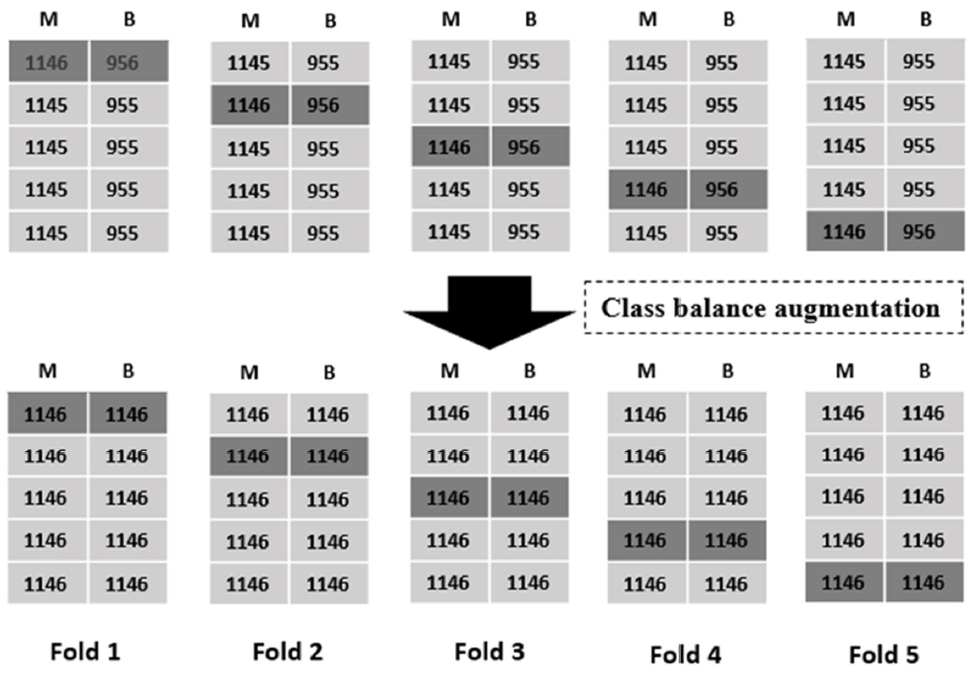
\includegraphics[width=0.90\textwidth]{2/figures/vitpaper2_part1.png}
		\caption[Balanceo de clases usando Aumento de Datos]{Balanceo de clases usando Aumento de Datos. \\
		Fuente: \cite{pr_ayana2023ViTtrasnferLMC}. \textit{Vision-Transformer-Based Transfer Learning for Mammogram Classification}.}
		\label{2:fig108}
	\end{center}
\end{figure}

Una vez obtenida la data ya balanceada, se realizó el preprocesamiento a las imágenes, específicamente, se redimensionó a las imágenes a 244 x 244 pixeles, esto debido a que el tamaño de las imágenes del conjunto de datos era variable. 

El diseño del modelo consiste inicialmente de la arquitectura de Vision Transformer. Se explica que siendo un modelo derivado de los convencionales transformer usados para el proceso del lenguaje natural o NLP donde las entradas son de una sola dimensión, los Vision Transformer se adaptaron para recibir entradas de dos dimensiones (imágenes). 

Específicamente, el modelo se encarga de dividir las entradas en pequeñas partes, también de dos dimensiones,conocidas como patches que finalmente servirán como entrada y serán pasada como word tokens, de igual forma que en un modelo transformer NLP. Aunque antes de proveer estos patches, se realizan los procesos de flattening, sequence imbedding, learnable embedding y patch embedding.

Además del bloque transformer, se tiene una parte de MLP encargada de la tarea de clasificación. Este posee una sola capa oculta y utiliza la función de activación GELU.

En el Figura \ref{2:fig109} se muestra la estructura del modelo implementado en la investigación.

\begin{figure}[H]
	\begin{center}
		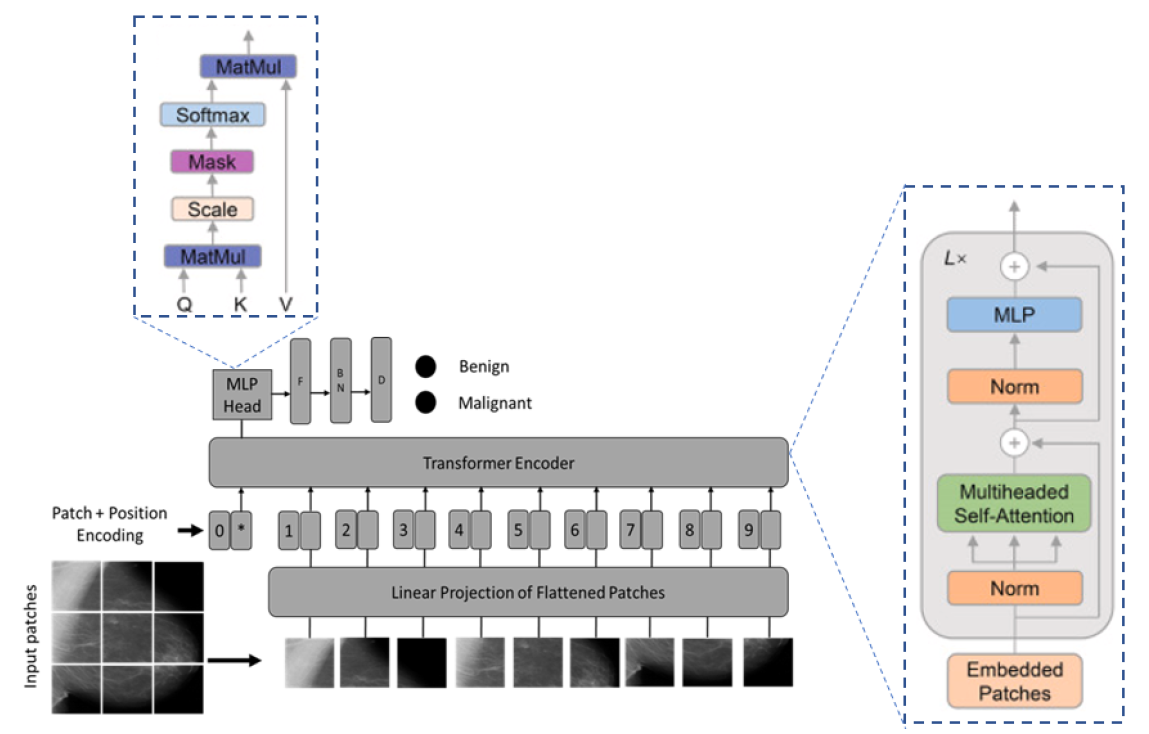
\includegraphics[width=1.00\textwidth]{2/figures/vitpaper2_part2.png}
		\caption[Estructura de ViT implementado]{Estructura de ViT implementado. \\
		Fuente: \cite{pr_ayana2023ViTtrasnferLMC}. \textit{Vision-Transformer-Based Transfer Learning for Mammogram Classification}.}
		\label{2:fig109}
	\end{center}
\end{figure}

El Transfer Learning fue aplicado en la investigación a través del uso de modelos de Vision Transformer pre-entrenados con el extenso conjunto de datos ImageNet, y posteriormente utilizados para entrenar el conjunto de datos de imágenes mamográficas. Es decir que se aprovechó el conocimiento de dichos modelos para la tarea final de clasificación de mamografías en benigno y maligno. Los modelos usados para este proceso fueron el Vision Transformer (ViT), Swin Transformer (Swin-T) y el Pyramid Vision Transformer (PVT).

El modelo Swin-T posee cuatro distintas versiones: Swin-base, Swin-tiny, Swin-small y Swin-large. Las variantes usadas en esta investigación fueron el Swin-small y Swin-base. Mientras que de las 4 versiones de PVT (PVT-tiny, PVT-small, PVT-medium y PVT-large), se usaron solo el PVT-medium y PVT-large.

Los modelos fueron entrenados con 50 épocas, una tasa de aprendizaje de 0.0001, optimizador Adam y un tamaño de lote de 64. Además, se dividió el conjunto de datos en 80\% para entrenamiento y 20\% para prueba.

Los Vision Transformer usaron GELU como función de activación, mientras que los CNN usaron ReLu. Ambos usaron el regularizador L2.

También se aplicó validación cruzada de 5 para lograr una mejor comparación en el rendimiento de los modelos.

Las métricas usadas para el proceso de evaluación de los modelos fueron el accuracy, AUC, F1-score, preicision, recall, el coeficiente de correlación de Matthew y el kappa score.

Se evaluó el método propuesto a través de 5 formas distintas: comparación de desempeño de los 3 modelos con Transfer Learning, comparación de los modelos Vision Transformer entrenados desde cero con el conjunto de datos de mamografías, comparación de Transfer Learning de Vision Transformer con los CNN, comparación de costo computacional de cada modelo Vision Transformer y, finalmente, se comparó el desempeño de los métodos desarrollados en esta investigación con otros que usaron el mismo conjunto de datos.

Como se muestra en la Tabla \ref{2:table7}, Tabla \ref{2:table8} y Tabla \ref{2:table9}, los 6 modelos Transfer Learning basados en arquitectura de Vision Transformer y entrenados con el conjunto de datos DDSM tuvieron un desempeño uniforme a través de todas la métricas.

\begin{table}[H]
	\caption[Resultado de los modelo ViT basados en Transfer Learning en el conjunto de datos DDSM (accuracy, AUC, f1-score)]{Resultado de los modelo ViT basados en Transfer Learning en el conjunto de datos DDSM (accuracy, AUC, f1-score).}
	\label{2:table7}
	\centering
	\small
	\begin{tabular}{m{3cm}m{3cm}m{2.4cm}m{2.5cm}m{2.5cm}}
		\specialrule{.1em}{.05em}{.05em}
		{Arquitectura} & {Modelo} & {Accuracy (95\%)} & {AUC (95\%)} & {F1 Score (95\%)}  \\
		\specialrule{.1em}{.05em}{.05em}
		\multirow{2}{3cm}{Vision Transformer} & {ViT-Base} & {$1 \pm 0$} & {$1 \pm 0$} & {$1 \pm 0$}  \\
		{} & {ViT-Large} & {$1 \pm 0$} & {$1 \pm 0$} & {$1 \pm 0$} \\
		\multirow{2}{3cm}{Swin Transformer} & {Swin-Small} & {$1 \pm 0$} & {$1 \pm 0$} & {$1 \pm 0$} \\
		{} & {Swim-Base} & {$1 \pm 0$} & {$1 \pm 0$} & {$1 \pm 0$} \\
		\multirow{2}{3cm}{Pyramid Vision Transformer} & {PVT-Medium} & {$1 \pm 0$} & {$1 \pm 0$} & {$1 \pm 0$} \\
		{} & {PVT-Large} & {$1 \pm 0$} & {$1 \pm 0$} & {$1 \pm 0$} \\
		\specialrule{.1em}{.05em}{.05em}
	\end{tabular}
	\begin{flushleft}	
		\small Fuente: \cite{pr_ayana2023ViTtrasnferLMC}. \textit{Vision-Transformer-Based Transfer Learning for Mammogram Classification}.
	\end{flushleft}
\end{table}

\begin{table}[H]
	\caption[Resultado de los modelo ViT basados en Transfer Learning en el conjunto de datos DDSM (precision, recall, MCC)]{Resultado de los modelo ViT basados en Transfer Learning en el conjunto de datos DDSM (precision, recall, MCC).}
	\label{2:table8}
	\centering
	\small
	\begin{tabular}{m{3cm}m{3cm}m{2.4cm}m{2.5cm}m{2.5cm}}
		\specialrule{.1em}{.05em}{.05em}
		{Arquitectura} & {Modelo} & {Precision (95\%)} & {Recall (95\%)} & {MCC (95\%)}  \\
		\specialrule{.1em}{.05em}{.05em}
		\multirow{2}{3cm}{Vision Transformer} & {ViT-Base} & {$1 \pm 0$} & {$1 \pm 0$} & {$1 \pm 0$}  \\
		{} & {ViT-Large} & {$1 \pm 0$} & {$1 \pm 0$} & {$1 \pm 0$} \\
		\multirow{2}{3cm}{Swin Transformer} & {Swin-Small} & {$1 \pm 0$} & {$1 \pm 0$} & {$1 \pm 0$} \\
		{} & {Swim-Base} & {$1 \pm 0$} & {$1 \pm 0$} & {$1 \pm 0$} \\
		\multirow{2}{3cm}{Pyramid Vision Transformer} & {PVT-Medium} & {$1 \pm 0$} & {$1 \pm 0$} & {$1 \pm 0$} \\
		{} & {PVT-Large} & {$1 \pm 0$} & {$1 \pm 0$} & {$1 \pm 0$} \\
		\specialrule{.1em}{.05em}{.05em}
	\end{tabular}
	\begin{flushleft}	
		\small Fuente: \cite{pr_ayana2023ViTtrasnferLMC}. \textit{Vision-Transformer-Based Transfer Learning for Mammogram Classification}.
	\end{flushleft}
\end{table}

\begin{table}[H]
	\caption[Resultado de los modelo ViT basados en Transfer Learning en el conjunto de datos DDSM (kappa)]{Resultado de los modelo ViT basados en Transfer Learning en el conjunto de datos DDSM (kappa).}
	\label{2:table9}
	\centering
	\small
	\begin{tabular}{m{3cm}m{3cm}m{2.4cm}}
		\specialrule{.1em}{.05em}{.05em}
		{Arquitectura} & {Modelo} & {Kappa (95\%)} \\
		\specialrule{.1em}{.05em}{.05em}
		\multirow{2}{3cm}{Vision Transformer} & {ViT-Base} & {$1 \pm 0$} \\
		{} & {ViT-Large} & {$1 \pm 0$} \\
		\multirow{2}{3cm}{Swin Transformer} & {Swin-Small} & {$1 \pm 0$}\\
		{} & {Swim-Base} & {$1 \pm 0$} \\
		\multirow{2}{3cm}{Pyramid Vision Transformer} & {PVT-Medium} & {$1 \pm 0$}\\
		{} & {PVT-Large} & {$1 \pm 0$}  \\
		\specialrule{.1em}{.05em}{.05em}
	\end{tabular}
	\begin{flushleft}	
		\small Fuente: \cite{pr_ayana2023ViTtrasnferLMC}. \textit{Vision-Transformer-Based Transfer Learning for Mammogram Classification}.
	\end{flushleft}
\end{table}

La Tabla \ref{2:table10}, Tabla \ref{2:table11} y Tabla \ref{2:table12} muestran los resultados de los modelos Vision Transformer inplementados desde cero y entrenados con el conjunto de datos DDSM.

\begin{table}[H]
	\caption[Resultado de los modelo ViT entrenados desde cero en el conjunto de datos DDSM (accuracy, AUC, f1-score)]{Resultado de los modelo ViT entrenados desde cero en el conjunto de datos DDSM (accuracy, AUC, f1-score).}
	\label{2:table10}
	\centering
	\small
	\begin{tabular}{m{3cm}m{3cm}m{2.4cm}m{2.5cm}m{2.5cm}}
		\specialrule{.1em}{.05em}{.05em}
		{Arquitectura} & {Modelo} & {Accuracy (95\%)} & {AUC (95\%)} & {F1 Score (95\%)}  \\
		\specialrule{.1em}{.05em}{.05em}
		\multirow{2}{3cm}{Vision Transformer} & {ViT-Base} & {$0.74 \pm 0.02$} & {$0.73 \pm 0.03$} & {$0.74 \pm 0.01$}  \\
		{} & {ViT-Large} & {$0.72 \pm 0.04$} & {$0.72 \pm 0.02$} & {$0.72 \pm 0.03$} \\
		\multirow{2}{3cm}{Swin Transformer} & {Swin-Small} & {$0.75 \pm 0.02$} & {$0.75 \pm 0.03$} & {$0.75 \pm 0.01$} \\
		{} & {Swim-Base} & {$0.76 \pm 0.01$} & {$0.75 \pm 0.02$} & {$0.75 \pm 0.02$} \\
		\multirow{2}{3cm}{Pyramid Vision Transformer} & {PVT-Medium} & {$0.78 \pm 0.02$} & {$0.77 \pm 0.02$} & {$0.78 \pm 0.01$} \\
		{} & {PVT-Large} & {$0.77 \pm 0.03$} & {$0.77 \pm 0.01$} & {$0.77 \pm 0.02$} \\
		\specialrule{.1em}{.05em}{.05em}
	\end{tabular}
	\begin{flushleft}	
		\small Fuente: \cite{pr_ayana2023ViTtrasnferLMC}. \textit{Vision-Transformer-Based Transfer Learning for Mammogram Classification}.
	\end{flushleft}
\end{table}

\begin{table}[H]
	\caption[Resultado de los modelo ViT entrenados desde cero en el conjunto de datos DDSM (precision, recall, MCC)]{Resultado de los modelo ViT entrenados desde cero en el conjunto de datos DDSM (precision, recall, MCC).}
	\label{2:table11}
	\centering
	\small
	\begin{tabular}{m{3cm}m{3cm}m{2.4cm}m{2.5cm}m{2.5cm}}
		\specialrule{.1em}{.05em}{.05em}
		{Arquitectura} & {Modelo} & {Precision (95\%)} & {Recall (95\%)} & {MCC (95\%)}  \\
		\specialrule{.1em}{.05em}{.05em}
		\multirow{2}{3cm}{Vision Transformer} & {ViT-Base} & {$0.74 \pm 0.01$} & {$0.74 \pm 0.01$} & {$0.73 \pm 0.03$}  \\
		{} & {ViT-Large} & {$0.72 \pm 0.04$} & {$0.72 \pm 0.03$} & {$0.71 \pm 0.02$} \\
		\multirow{2}{3cm}{Swin Transformer} & {Swin-Small} & {$0.75 \pm 0.02$} & {$0.75 \pm 0.02$} & {$0.74 \pm 0.03$} \\
		{} & {Swim-Base} & {$0.75 \pm 0.01$} & {$0.76 \pm 0.01$} & {$0.75 \pm 0.01$} \\
		\multirow{2}{3cm}{Pyramid Vision Transformer} & {PVT-Medium} & {$0.78 \pm 0.02$} & {$0.78 \pm 0.02$} & {$0.77 \pm 0.01$} \\
		{} & {PVT-Large} & {$0.77 \pm 0.02$} & {$0.77 \pm 0.02$} & {$0.77 \pm 0.01$} \\
		\specialrule{.1em}{.05em}{.05em}
	\end{tabular}
	\begin{flushleft}	
		\small Fuente: \cite{pr_ayana2023ViTtrasnferLMC}. \textit{Vision-Transformer-Based Transfer Learning for Mammogram Classification}.
	\end{flushleft}
\end{table}

\begin{table}[H]
	\caption[Resultado de los modelo ViT entrenados desde cero en el conjunto de datos DDSM (kappa)]{Resultado de los modelo ViT entrenados desde cero en el conjunto de datos DDSM (kappa).}
	\label{2:table12}
	\centering
	\small
	\begin{tabular}{m{3cm}m{3cm}m{2.4cm}}
		\specialrule{.1em}{.05em}{.05em}
		{Arquitectura} & {Modelo} & {Kappa (95\%)} \\
		\specialrule{.1em}{.05em}{.05em}
		\multirow{2}{3cm}{Vision Transformer} & {ViT-Base} & {$0.73 \pm 0.02$} \\
		{} & {ViT-Large} & {$0.72 \pm 0.01$} \\
		\multirow{2}{3cm}{Swin Transformer} & {Swin-Small} & {$0.74 \pm 0.02$}\\
		{} & {Swim-Base} & {$0.75 \pm 0.02$} \\
		\multirow{2}{3cm}{Pyramid Vision Transformer} & {PVT-Medium} & {$0.77 \pm 0.02$}\\
		{} & {PVT-Large} & {$0.77 \pm 0.01$}  \\
		\specialrule{.1em}{.05em}{.05em}
	\end{tabular}
	\begin{flushleft}	
		\small Fuente: \cite{pr_ayana2023ViTtrasnferLMC}. \textit{Vision-Transformer-Based Transfer Learning for Mammogram Classification}.
	\end{flushleft}
\end{table}

Se puede observar que el modelo PVT-medium obtuvo un mejor desempeño comparado a los demás modelos. Sin embargo, estos resultados se mantienen muy por debajo de los presentados anteriormente.

Finalmente, también se obtuvieron resultados de los experimentos de Transfer Learning con modelos CNN y el conjunto de datos DDSM. Estos se muestran en la Tabla \ref{2:table13}, Tabla \ref{2:table14} y Tabla \ref{2:table15}.

\begin{table}[H]
	\caption[Resultado de los modelos CNN basados en Transfer Learning en el conjunto de datos DDSM (accuracy, AUC, f1-score)]{Resultado de los modelos CNN basados en Transfer Learning en el conjunto de datos DDSM (accuracy, AUC, f1-score).}
	\label{2:table13}
	\centering
	\small
	\begin{tabular}{m{3cm}m{3cm}m{2.4cm}m{2.5cm}m{2.5cm}}
		\specialrule{.1em}{.05em}{.05em}
		{Arquitectura} & {Modelo} & {Accuracy (95\%)} & {AUC (95\%)} & {F1 Score (95\%)}  \\
		\specialrule{.1em}{.05em}{.05em}
		\multirow{2}{3cm}{ResNet} & {ResNet50} & {$0.95 \pm 0.01$} & {$0.96 \pm 0.01$} & {$0.95 \pm 0.01$}  \\
		{} & {ResNet101} & {$0.95 \pm 0.01$} & {$0.95 \pm 0.02$} & {$0.95 \pm 0.01$} \\
		\multirow{2}{3cm}{EfficientNet} & {EfficientNetB0} & {$0.94 \pm 0.02$} & {$0.94 \pm 0.01$} & {$0.94 \pm 0.01$} \\
		{} & {EfficientNetB2} & {$0.95 \pm 0.01$} & {$0.95 \pm 0.01$} & {$0.95 \pm 0.01$} \\
		\multirow{2}{3cm}{InceptionNet} & {InceptionNetV2} & {$0.93 \pm 0.02$} & {$0.93 \pm 0.01$} & {$0.93 \pm 0.02$} \\
		{} & {InceptionNetV3} & {$0.94 \pm 0.01$} & {$0.94 \pm 0.01$} & {$0.94 \pm 0.01$} \\
		\specialrule{.1em}{.05em}{.05em}
	\end{tabular}
	\begin{flushleft}	
		\small Fuente: \cite{pr_ayana2023ViTtrasnferLMC}. \textit{Vision-Transformer-Based Transfer Learning for Mammogram Classification}.
	\end{flushleft}
\end{table}

\begin{table}[H]
	\caption[Resultado de los modelos CNN basados en Transfer Learning en el conjunto de datos DDSM (precision, recall, MCC)]{Resultado de los modelos CNN basados en Transfer Learning en el conjunto de datos DDSM (precision, recall, MCC).}
	\label{2:table14}
	\centering
	\small
	\begin{tabular}{m{3cm}m{3cm}m{2.4cm}m{2.5cm}m{2.5cm}}
		\specialrule{.1em}{.05em}{.05em}
		{Arquitectura} & {Modelo} & {Precision (95\%)} & {Recall (95\%)} & {MCC (95\%)}  \\
		\specialrule{.1em}{.05em}{.05em}
		\multirow{2}{3cm}{ResNet} & {ResNet50} & {$0.95 \pm 0.01$} & {$0.95 \pm 0.01$} & {$0.94 \pm 0.01$}  \\
		{} & {ResNet101} & {$0.95 \pm 0.01$} & {$0.95 \pm 0.01$} & {$0.94 \pm 0.02$} \\
		\multirow{2}{3cm}{EfficientNet} & {EfficientNetB0} & {$0.94 \pm 0.01$} & {$0.94 \pm 0.01$} & {$0.93 \pm 0.03$} \\
		{} & {EfficientNetB2} & {$0.95 \pm 0.01$} & {$0.95 \pm 0.01$} & {$0.95 \pm 0.01$} \\
		\multirow{2}{3cm}{InceptionNet} & {InceptionNetV2} & {$0.93 \pm 0.02$} & {$0.93 \pm 0.02$} & {$0.93 \pm 0.03$} \\
		{} & {InceptionNetV3} & {$0.94 \pm 0.01$} & {$0.94 \pm 0.01$} & {$0.93 \pm 0.02$} \\
		\specialrule{.1em}{.05em}{.05em}
	\end{tabular}
	\begin{flushleft}	
		\small Fuente: \cite{pr_ayana2023ViTtrasnferLMC}. \textit{Vision-Transformer-Based Transfer Learning for Mammogram Classification}.
	\end{flushleft}
\end{table}

\begin{table}[H]
	\caption[Resultado de los modelos CNN basados en Transfer Learning en el conjunto de datos DDSM (kappa)]{Resultado de los modelos CNN basados en Transfer Learning en el conjunto de datos DDSM (kappa).}
	\label{2:table15}
	\centering
	\small
	\begin{tabular}{m{3cm}m{3cm}m{2.4cm}}
		\specialrule{.1em}{.05em}{.05em}
		{Arquitectura} & {Modelo} & {Kappa (95\%)} \\
		\specialrule{.1em}{.05em}{.05em}
		\multirow{2}{3cm}{ResNet} & {ResNet50} & {$0.94 \pm 0.02$} \\
		{} & {ResNet101} & {$0.94 \pm 0.02$} \\
		\multirow{2}{3cm}{EfficientNet} & {EfficientNetB0} & {$0.93 \pm 0.02$}\\
		{} & {EfficientNetB2} & {$0.95 \pm 0.01$} \\
		\multirow{2}{3cm}{InceptionNet} & {InceptionNetV2} & {$0.92 \pm 0.02$}\\
		{} & {InceptionNetV3} & {$0.93 \pm 0.02$}  \\
		\specialrule{.1em}{.05em}{.05em}
	\end{tabular}
	\begin{flushleft}	
		\small Fuente: \cite{pr_ayana2023ViTtrasnferLMC}. \textit{Vision-Transformer-Based Transfer Learning for Mammogram Classification}.
	\end{flushleft}
\end{table}


El desempeño de los modelos CNN también se encuentran por debajo de los Vision Transformer presentados inicialmente. 

\cite{pr_manzari2023MedViTGMIC} nos menciona que dentro del análisis de imágenes médicas, la tarea de clasificación es crucial. Por ello, este se ha visto beneficiado constantemente de novedosos sistemas de diagnóstico asistido, siendo los de mayor desempeño aquellos basados en Redes Neuronales Convolucionales (CNN), pues ofrecen predicciones cada vez más precisas incluso comparándose con los médicos. Sin embargo, estos también tienen algunas desventajas o dificultades, principalmente lo relacionado a su capacidad de aprendizaje de dependencias a largo alcance en conjuntos de datos visuales, esto debido al conocido sesgo local de las CNN.

En este contexto, las arquitecturas basadas en transformers y su mecanismo de autoatención, han demostrado ser capaces de solucionar estas desventajas de las CNN. Esto debido a su capacidad de modelar las dependencias a largo alcance de los datos, convirtiéndolos así en modelos superiores a las arquitectura de CNN, aunque con mayor necesidad en cantidad de datos de entrenamiento, recursos computacionales y tiempo.

A pesar de los beneficios que pueden traer las arquitecturas transformer frente a los CNN, estos están muy limitadas en su uso en las tareas de análisis de imágenes médicas. Esto es debido principalmente a sus desventajas ya mencionadas (alta necesidad de recursos computacionales y tiempo), pues en el entorno clínico, la eficiencia y la velocidad es de suma importancia para realizar pre-diagnósticos satisfactorios.

Los altos requerimientos de los transformer traen consigo grandes dificultades, impidiendo que estos puedan ser usados en situaciones clínicas reales. Además, también existe el problema de la suposición de una distribución similar en los datos que se van a ingresar al modelo; sin embargo, se sabe que esto no siempre se cumple en el entorno real, debido a que las imágenes médicas son capturadas a través de distintos dispositivos, diversos protocolos y diferentes lugares. Esta discrepancia en los datos puede generar que el rendimiento del modelo caiga considerablemente.

Ante este problema, la investigación propone un nueva arquitectura basada en transformer con capacidad de generalización de distintos tipos de imágenes médicas como las tomografías computarizadas, rayos X y ultrasonido. Su estructura se caracteriza por ser híbrida jerárquica, poseer patch embedding y poseer convoluciones y bloques de transformer. Además, se incluyó en la arquitectura del transformer un bloque de atención convolucional multi-cabezal con el fin de mejorar la capacidad de aprendizaje de representación local, incluso este permitió reducir la complejidad computacional comparado con un modelo transformer convencional.

Comparándolo con los CNN, el modelo desarrollado también demostró una capacidad superior en la tarea de predicción, al mismo tiempo que poseía menor complejidad.

De forma generar el modelo MedViT, propuesto en esta investigación, tiene como objetivo lograr una arquitectura híbrida capaz de desempeñarse en la tarea de clasificación de imágenes médicas, a través de la combinación de bloques de convolución y transformer, además de estar también compuesto por capas de path embedding, siguiendo así una tradicional arquitectura piramidal jerárquica.

Los bloques principales de modelo son el Efficient Convolution Block (ECB) y el Local Transformer Block (LTB). Estos se encargan de capturar las dependencias de los datos de entrada a largo y corto plazo.

También se propuso una nueva técnica de Aumento de Datos denominada Patch Momentum Charge (PMC) con el objetivo de mejorar el rendimiento del modelo.

Los experimentos se realizaron con 12 distintos conjuntos de datos de la categoría imágenes médicas. Todos estos se encontraron en MedMINIST, y conforman imágenes de tomografías computarizadas, rayos X, ultrasonido y tomografías de coherencia óptica (OCT). Esta variedad de datos permiten el entrenamiento de modelos en tareas de clasificación.

De forma específica, los conjuntos de datos usados fueron el PathMNIST (posee 100 000 image patches categorizadas en 9 clases distintas relacionadas a patologías en el colon), ChestMNIST (posee 112 120 imágenes frontales de rayos X de 32 717 pacientes dividida en 14 clases distintas de enfermedades de tórax), DermaMNIST (posee 10 015 imágenes dermatoscópicas recopiladas de distintas fuentes y divididas en 7 clases relacionadas a enfermedades de la piel), OCTMNIST (consta de 109 309 imágenes de OCT recopiladas de pacientes con enfermedades de la retina y dividida en 4 clases distintas), PneumoniaMNIST (recopila 5 856 imágenes radiográficas pediátricas de tórax categorizadas en 2 clases que indican presencia o no de neumonía), RetinaMNIST (provee 1 600 imágenes de fondo de retina de 628 pacientes y se divide en 5 clases que indican la gravedad de la enfermedad de retinopatía diabética), TissueMNIST (dividida en 8 clases, este conjunto de datos está compuesto de 236 386 imágenes segmentadas de tejidos de corteza renal), BloodMNIST (consta de 17 092 imágenes de células sanguíneas categorizadas en 8 clases), BreastMNIST (categorizada en las clases de benigno, maligno y normal, este conjunto de datos posee 780 ecografías mamarias) y OrganMNIST (consta de imágenes de tomografías computarizadas abdominales divididas en 11 clases en sus 3 versiones: Axial, Coronal y Sagital).

En la etapa de entrenamiento del modelo con los 12 conjuntos de datos descritos anteriormente, se siguieron los mismos ajustes de entrenamiento de MedMNISTv2. Se usaron 100 épocas con un tamaño de lote de 128 y se aplicó el redimensionado a las imágenes para obtener la forma de 224 x 224 pixeles. Además, se usó el optimizar AdamW con una tasa de aprendizaje de 0.0001.

MedViT consiste en 3 distintas arquitecturas definidas por su tamaño: MedViT-T, MedViT-S y MedViT-L. Estas fueron entrenadas de forma separada con cada uno de los conjuntos de datos. También se incluyó el Aumento de Datos a través de PMC.en la etapa de entrenamiento.

Las métricas usadas para evaluar las 3 versiones del modelo MedViT fueron el accuracy y la curva ROC. Esta elección fue debido a que el experimento se llevó a cabo en varios conjuntos de datos distintos entre sí. 

De los resultados mostrados en la Tabla \ref{2:table16}, Tabla \ref{2:table17}, Tabla \ref{2:table18} y Tabla \ref{2:table19}, los modelos MedViT superan, de forma general, en gran medida a los modelos basados en CNN en la misma tarea. Esto lleva a concluir que el modelo demuestra una alta capacidad de generalización en imágenes médicas.

\begin{table}[H]
	\caption[Comparación de resultados de los modelos MedViT con los CNN y AutoML (PathMNIST, ChestMNIST y DermaMNIST)]{Comparación de resultados de los modelos MedViT con los CNN y AutoML (PathMNIST, ChestMNIST y DermaMNIST).}
	\label{2:table16}
	\centering
	\small
	\begin{tabular}{lcccccc}
		\specialrule{.1em}{.05em}{.05em}
		\multirow{2}{3cm}{Métodos} & \multicolumn{2}{l}{PathMNIST} & \multicolumn{2}{l}{ChestMNIST} & \multicolumn{2}{l}{DermaMNIST} \\
		{} & {AUC} & {ACC} & {AUC} & {ACC} & {AUC} & {ACC} \\
		\specialrule{.1em}{.05em}{.05em}
		{ResNet-18 (28)} & {0.983} & {0.907} & {0.768} & {0.947} & {0.917} & {0.735} \\
		{RestNet-18 (224)} & {0.989} & {0.909} & {0.773} & {0.947} & {0.920} & {0.754} \\
		{ResNet-50 (28)} & {0.990} & {0.911} & {0.769} & {0.947} & {0.913} & {0.735} \\
		{RestNet-50 (224)} & {0.989} & {0.892} & {0.773} & {0.948} & {0.912} & {0.731} \\
		{auto-sklearn} & {0.934} & {0.716} & {0.649} & {0.779} & {0.902} & {0.719} \\
		{AutoKeras} & {0.959} & {0.834} & {0.742} & {0.937} & {0.915} & {0.749} \\
		{Google AutoML} & {0.944} & {0.728} & {0.778} & {0.948} & {0.914} & {0.768} \\
		{MedVIT-T (224)} & {0.994} & {0.938} & {0.786} & {0.956} & {0.914} & {0.768} \\
		{MedVIT-S (224)} & {0.993} & {0.942} & {0.791} & {0.954} & {0.937} & {0.780} \\
		{MedVIT-L (224)} & {0.984} & {0.933} & {0.805} & {0.959} & {0.920} & {0.773} \\
		\specialrule{.1em}{.05em}{.05em}
	\end{tabular}
	\begin{flushleft}	
		\small Fuente: \cite{pr_manzari2023MedViTGMIC}. \textit{MedViT: A robust vision transformer for generalized medical image classification}.
	\end{flushleft}
\end{table}

\begin{table}[H]
	\caption[Comparación de resultados de los modelos MedViT con los CNN y AutoML (OCTMNIST, PneumoniaMNIST y RetinaMNIST)]{Comparación de resultados de los modelos MedViT con los CNN y AutoML (OCTMNIST, PneumoniaMNIST y RetinaMNIST).}
	\label{2:table17}
	\centering
	\small
	\begin{tabular}{lcccccc}
		\specialrule{.1em}{.05em}{.05em}
		\multirow{2}{3cm}{Métodos} & \multicolumn{2}{l}{OCTMNIST} & \multicolumn{2}{l}{PneumoniaMNIST} & \multicolumn{2}{l}{RetinaMNIST} \\
		{} & {AUC} & {ACC} & {AUC} & {ACC} & {AUC} & {ACC} \\
		\specialrule{.1em}{.05em}{.05em}
		{ResNet-18 (28)} & {0.943} & {0.743} & {0.944} & {0.854} & {0.717} & {0.524} \\
		{RestNet-18 (224)} & {0.958} & {0.763} & {0.956} & {0.864} & {0.710} & {0.493} \\
		{ResNet-50 (28)} & {0.952} & {0.762} & {0.948} & {0.954} & {0.726} & {0.528} \\
		{RestNet-50 (224)} & {0.958} & {0.776} & {0.962} & {0.884} & {0.716} & {0.511} \\
		{auto-sklearn} & {0.887} & {0.601} & {0.942} & {0.855} & {0.690} & {0.515} \\
		{AutoKeras} & {0.955} & {0.763} & {0.947} & {0.878} & {0.719} & {0.503} \\
		{Google AutoML} & {0.963} & {0.771} & {0.991} & {0.946} & {0.750} & {0.531} \\
		{MedVIT-T (224)} & {0.961} & {0.767} & {0.993} & {0.949} & {0.752} & {0.534} \\
		{MedVIT-S (224)} & {0.960} & {0.982} & {0.995} & {0.961} & {0.773} & {0.561} \\
		{MedVIT-L (224)} & {0.945} & {0.761} & {0.991} & {0.921} & {0.754} & {0.552} \\
		\specialrule{.1em}{.05em}{.05em}
	\end{tabular}
	\begin{flushleft}	
		\small Fuente: \cite{pr_manzari2023MedViTGMIC}. \textit{MedViT: A robust vision transformer for generalized medical image classification}.
	\end{flushleft}
\end{table}

\begin{table}[H]
	\caption[Comparación de resultados de los modelos MedViT con los CNN y AutoML (BreastMNIST, BloodMNIST y TissueMNIST)]{Comparación de resultados de los modelos MedViT con los CNN y AutoML (BreastMNIST, BloodMNIST y TissueMNIST).}
	\label{2:table18}
	\centering
	\small
	\begin{tabular}{lcccccc}
		\specialrule{.1em}{.05em}{.05em}
		\multirow{2}{3cm}{Métodos} & \multicolumn{2}{l}{BreastMNIST} & \multicolumn{2}{l}{BloodMNIST} & \multicolumn{2}{l}{TissueMNIST} \\
		{} & {AUC} & {ACC} & {AUC} & {ACC} & {AUC} & {ACC} \\
		\specialrule{.1em}{.05em}{.05em}
		{ResNet-18 (28)} & {0.901} & {0.863} & {0.998} & {0.958} & {0.930} & {0.676} \\
		{RestNet-18 (224)} & {0.891} & {0.833} & {0.998} & {0.963} & {0.933} & {0.681} \\
		{ResNet-50 (28)} & {0.857} & {0.812} & {0.997} & {0.956} & {0.931} & {0.680} \\
		{RestNet-50 (224)} & {0.866} & {0.842} & {0.997} & {0.950} & {0.932} & {0.680} \\
		{auto-sklearn} & {0.836} & {0.803} & {0.984} & {0.878} & {0.828} & {0.532} \\
		{AutoKeras} & {0.871} & {0.831} & {0.998} & {0.961} & {0.941} & {0.703} \\
		{Google AutoML} & {0.919} & {0.861} & {0.998} & {0.966} & {0.924} & {0.673} \\
		{MedVIT-T (224)} & {0.934} & {0.896} & {0.996} & {0.950} & {0.943} & {0.703} \\
		{MedVIT-S (224)} & {0.938} & {0.897} & {0.997} & {0.951} & {0.952} & {0.731} \\
		{MedVIT-L (224)} & {0.929} & {0.883} & {0.996} & {0.954} & {0.935} & {0.699} \\
		\specialrule{.1em}{.05em}{.05em}
	\end{tabular}
	\begin{flushleft}	
		\small Fuente: \cite{pr_manzari2023MedViTGMIC}. \textit{MedViT: A robust vision transformer for generalized medical image classification}.
	\end{flushleft}
\end{table}

\begin{table}[H]
	\caption[Comparación de resultados de los modelos MedViT con los CNN y AutoML (OrganMNIST, OrganCMNIST y OrganSMNIST)]{Comparación de resultados de los modelos MedViT con los CNN y AutoML (OrganMNIST, OrganCMNIST y OrganSMNIST).}
	\label{2:table19}
	\centering
	\small
	\begin{tabular}{lcccccc}
		\specialrule{.1em}{.05em}{.05em}
		\multirow{2}{3cm}{Métodos} & \multicolumn{2}{l}{OrganMNIST} & \multicolumn{2}{l}{OrganCMNIST} & \multicolumn{2}{l}{OrganSMNIST} \\
		{} & {AUC} & {ACC} & {AUC} & {ACC} & {AUC} & {ACC} \\
		\specialrule{.1em}{.05em}{.05em}
		{ResNet-18 (28)} & {0.997} & {0.935} & {0.992} & {0.900} & {0.972} & {0.782} \\
		{RestNet-18 (224)} & {0.998} & {0.951} & {0.994} & {0.920} & {0.974} & {0.778} \\
		{ResNet-50 (28)} & {0.997} & {0.935} & {0.992} & {0.905} & {0.972} & {0.770} \\
		{RestNet-50 (224)} & {0.998} & {0.947} & {0.993} & {0.911} & {0.975} & {0.785} \\
		{auto-sklearn} & {0.963} & {0.762} & {0.976} & {0.829} & {0.845} & {0.672} \\
		{AutoKeras} & {0.994} & {0.905} & {0.990} & {0.879} & {0.974} & {0.813} \\
		{Google AutoML} & {0.990} & {0.886} & {0.988} & {0.877} & {0.964} & {0.749} \\
		{MedVIT-T (224)} & {0.995} & {0.931} & {0.991} & {0.901} & {0.972} & {0.789} \\
		{MedVIT-S (224)} & {0.996} & {0.928} & {0.993} & {0.916} & {0.987} & {0.805} \\
		{MedVIT-L (224)} & {0.997} & {0.943} & {0.994} & {0.922} & {0.973} & {0.806} \\
		\specialrule{.1em}{.05em}{.05em}
	\end{tabular}
	\begin{flushleft}	
		\small Fuente: \cite{pr_manzari2023MedViTGMIC}. \textit{MedViT: A robust vision transformer for generalized medical image classification}.
	\end{flushleft}
\end{table}

\cite{pr_regmi2023ViTChestXray} nos menciona la gran importancia que tiene el análisis de imágenes médicas para la detección a tiempo de enfermedades potencialmente mortales. Los radiólogos y personal clínico realizan esta importante tarea en la gran mayoría de los casos; sin embargo, sus interpretaciones de las imágenes no siempre están en lo correcto debido a que su análisis muchas veces está condicionado por el mismo observador, llevando a que los niveles de precisión para interpretar este tipo de datos no sean tan altos.

Esta tarea de interpretación de imágenes médicas es aun más importante en los casos de una alta necesidad de detectar a tiempo alguna enfermedad; por ejemplo, las relacionadas a los pulmones o las enfermedades gastrointestinales que pueden no causar daño como el reflujo ácido u otras de grave impacto como el cáncer de colon. Una detección a tiempo de estos permite aplicar los tratamientos debidos y así, consecuentemente, mejorar la calidad de vida de los pacientes. En este contexto, los sistemas de diagnóstico asistido por computadora (CAD por sus siglas en inglés) han demostrado ser de gran ayuda para los médicos y expertos clínicos en la tarea de realizar diagnósticos tempranos.

La capacidad de las Redes Neuronales Convolucionales (CNN) de poder adaptarse en detectar distintas característica de un conjunto de datos han permitido su desarrollo en el campo médico, específicamente en las tareas de segmentación, clasificación, registro y reconstrucción de imágenes médicas.

Otra técnica popular que va tomando cada vez más mayor importancia son los Vision Transformer (ViT) capaces también de desempeñarse satisfactoriamente en las tareas de clasificación de imágenes, a pesar de ser basados en los originales transformers especializados en tareas relacionadas a texto.

Otro tipo de arquitectura basada en transformer son los Data-Efficient Image Transformer (DeiT), una versión de nuevos de los ViT caracterizados por su baja dependencia a los datos a través de su enfoque maestro-estudiante.

En esta investigación se presentan distintas arquitecturas basadas en CNN y Transformer para la clasificación de radiografías de tórax en distintos tipos de enfermedades relacionadas. Específicamente, se usaron los modelos DeiT, ViT y Ensemble, este último basado en otros modelos CNN. También se aplicó Transfer Learning junto a modelos CNN previamente entrenados. Finalmente todos los modelos fueron comparados en la misma tarea de clasificación de imágenes.

Se usaron distintas versiones de ViT (ViT-B/16, ViT-L/16, ViT-L/32) pre-entrenados con el conjunto de datos ImageNet-21k. 

La diferencia principal entre ViT-L/16 y ViT-L/32 radica en el tamaño de los patch de entrada que permiten, siendo para el primer caso un patch de tamaño 16x16, mientras que el segundo un patch de 32 x 32. Todos estos modelos pasaron por un proceso de fine-tuning con 3 conjuntos de datos.

El primer conjunto de datos usado fue el Chest X-ray dataset que consistía en 7 135 imágenes, divididas en 4 clases (COVID-19, neumonía, tuberculosis y normal).

El conjunto de datos Kvasir consiste de 1 000 imágenes en cada una de las 8 clases existentes.

El último conjunto de datos, Kvasir-Capsule dataset consiste de 44 228 imágenes de endoscopía divididas en 13 clases. La cantidad de imágenes varía en cada clase del conjunto de datos, lo cual lo vuelve altamente imbalanceado.

En la Tabla \ref{2:table20} se resumen las características de los 3 conjuntos de datos.


\begin{table}[H]
	\caption[Resumen de características de los conjuntos de datos]{Resumen de características de los conjuntos de datos.}
	\label{2:table20}
	\centering
	\small
	\begin{tabular}{m{2.5cm}m{1.5cm}m{2.5cm}m{1.5cm}m{1.5cm}m{1.5cm}m{2.5cm}}
		\specialrule{.1em}{.05em}{.05em}
		{Dataset} & {N° de Imágenes} & {Tamaño de entrada} & {Entren.} & {Val.} & {Prue.} & {Aplicación} \\
		\specialrule{.1em}{.05em}{.05em}
		{Chest X-ray dataset} & {7135} & {variable} & {5693} & {671} & {771} & {Enfermedad pulmonar} \\
		{Kvasir dataset} & {8000} & {720 x 556} & {6400} & {800} & {800} & {Endoscopía} \\
		{Kvasir-Capsule} & {44152} & {336 x 336} & {19280} & {4820} & {23061} & {Enfermedad intestinal} \\
		\specialrule{.1em}{.05em}{.05em}
	\end{tabular}
	\begin{flushleft}	
		\small Fuente: \cite{pr_regmi2023ViTChestXray}. \textit{Vision transformer for efficient chest X-ray and gastrointestinal image classification}.
	\end{flushleft}
\end{table}


El modelo ViT base (ViT-B) está compuesto por 12 bloques transformer con módulos de autoatención de 12 cabezas, permitiendo un total de 86 millones de parámetros entrenables.

El modelo ViT large (ViT-L) consiste de 24 bloques transformer con módulos de autoatención de 16 cabezas, formando así 307 millones de parámetros entrenables.

Las imágenes del conjunto de datos Chest X-ray fueron redimensionadas a 224 x 224 pixeles. Esto también se aplicó al conjunto de datos Kvasir. 

En el caso de las imágenes de Kvasir-Capsule, estas tuvieron que ser redimensionadas a 64 x 64 pixeles.

Se usaron dos modelos de DeiT: DeiT-Ti y DeiT-B 384. El primero de estos permitía imágenes de 224 x 224 de resolución; mientras que el segundo, 384 x 384.

Todos los conjuntos de datos fueron divididos en data de entrenamiento, validación y prueba.

Además, se aplicaron distintas técnicas de Aumento de Datos para cada uno de los conjuntos de datos. En el caso de Chest X-ray se aplicó el reescalado, cambio de brillo, desplazamiento vertical y vertical, y zoom de forma aleatoria. Para el conjunto de datos Kvasir, se alteró el brillo de las imágenes, se rotaron y se dieron vuelta de manera vertical. Finalmente, para Kvasir-Capsule, se aplicó rotación, se dio vuelta a las imágenes de manera horizontal y vertical.

Los modelos CNN pre-entrenados que se usaron fueron el DenseNet201, DenseNet121, InceptionRestNetV2, Xception, MovileNetV2 y el Ensemble que combinaba DenseNet201 y DenseNet121.

Se probaron varios hiper-parámetros a través de prueba y error. Además, en el caso del conjunto de datos de Chest X-ray y Kvasir, se usó la función de pérdida categorical cross-entropy. Con Kvasir-Capsule, se usó el Focal Loss debido al desbalance de los datos en cada clase.

Las métricas usadas para evaluar la capacidad de clasificación de los modelos fueron el Matthews Correlation Coefficient (MCC), Frames Per Second (FPS), precision, F1-score, recall y accuracy.

El precision utilizado fue la media ponderada, esto pues es un método que asigna pesos de acuerdo a la cantidad de observaciones en cada clase, volviéndolo ideal para conjuntos de datos desbalanceados. Además, también se obtiene la desviación estándar del Recall, F1-score y Precision con el fin de verificar la variabilidad de los resultados.

Se realizó la prueba t por pares para comparar los resultados con la métrica MCC del modelo con mejor rendimiento.

Los resultados de los experimentos se muestran en la Tabla \ref{2:table21}, Tabla \ref{2:table22} y Tabla \ref{2:table23}.

\begin{table}[H]
	\caption[Resultados con el conjunto de datos Chest X-ray]{Resultados con el conjunto de datos Chest X-ray.}
	\label{2:table21}
	\centering
	\small
	\begin{tabular}{m{2.5cm}m{1.5cm}m{1.5cm}m{1.5cm}m{1.5cm}m{1.5cm}m{1.5cm}m{1.5cm}}
		\specialrule{.1em}{.05em}{.05em}
		{Método} & {Precision} & {Recall} & {F1-score} & {Acc.} & {MCC} & {P-val.} & {FPS}  \\
		\specialrule{.1em}{.05em}{.05em}
		{DenseNet201 + DenseNet121} & {$0.9345 \pm 0.0324$} & {$0.9326 \pm 0.0584$} & {$0.9319 \pm 0.0236$} & {0.9326} & {0.8931} & {1.24e-03} & {16.08} \\
		{DenseNet201} & {$0.9169 \pm 0.0358$} & {$0.9157 \pm 0.0538$} & {$0.9150 \pm 0.0195$} & {0.9157} & {0.8658} & {8.41e-05} & {22.47} \\
		{DenseNet121} & {$0.9314 \pm 0.0358$} & {$0.9287 \pm 0.0678$} & {$0.9277 \pm 0.0370$} & {0.9287} & {0.8878} & {3.37e-04} & {26.15} \\
		{Incep.RestNetV2} & {$0.9415\pm 0.0358$} & {$0.9403 \pm 0.0678$} & {$0.9400 \pm 0.0370$} & {0.9287} & {0.9052} & {1.18e-04} & {20.48} \\
		{Xception} & {$0.9380 \pm 0.0324$} & {$0.9377 \pm 0.0461$} & {$0.9375 \pm 0.0358$} & {0.9377} & {0.9010} & {4.80e-05} & {21.34} \\
		{MobileNetV2} & {$0.9133 \pm 0.0625$} & {$0.9092 \pm 0.0508$} & {$0.9099 \pm 0.0401$} & {0.9092} & {0.8567} & {8.96e-04} & {21.85} \\
		{DeiT-Ti} & {$0.9266 \pm 0.0453$} & {$0.9261 \pm 0.0326$} & {$0.9262 \pm 0.0368$} & {0.9261} & {0.8821} & {3.37e-04} & {25.84} \\
		{DeiT-B 384} & {$0.9332 \pm 0.0592$} & {$0.9300 \pm 0.0728$} & {$0.9291 \pm 0.0272$} & {0.9300} & {0.8899} & {1.10e-03} & {16.75} \\
		{ViT-L/32} & {$0.9527 \pm 0.0362$} & {$0.9520 \pm 0.0301$} & {$0.9521 \pm 0.0277$} & {0.9520} & {0.9236} & {3.83e-02} & {11.49} \\
		{ViT-L/16} & {$0.9533 \pm 0.0202$} & {$0.9533 \pm 0.0301$} & {$0.9532 \pm 0.0225$} & {0.9533} & {0.9259} & {-} & {11.20} \\
		{ViT-B/16} & {$0.9291 \pm 0.0592$} & {$0.9248 \pm 0.0728$} & {$0.9248 \pm 0.0272$} & {0.9248} & {0.8813} & {3.77e-04} & {20.74} \\
		\specialrule{.1em}{.05em}{.05em}
	\end{tabular}
	\begin{flushleft}	
		\small Fuente: \cite{pr_regmi2023ViTChestXray}. \textit{Vision transformer for efficient chest X-ray and gastrointestinal image classification}.
	\end{flushleft}
\end{table}

\begin{table}[H]
	\caption[Resultados con el conjunto de datos Kvasir]{Resultados con el conjunto de datos Kvasir.}
	\label{2:table22}
	\centering
	\small
	\begin{tabular}{m{2.5cm}m{1.5cm}m{1.5cm}m{1.5cm}m{1.5cm}m{1.5cm}m{1.5cm}m{1.5cm}}
		\specialrule{.1em}{.05em}{.05em}
		{Método} & {Precision} & {Recall} & {F1-score} & {Acc.} & {MCC} & {P-val.} & {FPS}  \\
		\specialrule{.1em}{.05em}{.05em}
		{DenseNet201 + DenseNet121} & {$0.9284 \pm 0.0559$} & {$0.9263 \pm 0.0711$} & {$0.9258 \pm 0.0538$} & {0.9263} & {0.9161} & {2.60e-01} & {12.32} \\
		{DenseNet201} & {$0.9262 \pm 0.0467$} & {$0.9250 \pm 0.0628$} & {$0.9246 \pm 0.0472$} & {0.9250} & {0.9146} & {1.52e-01} & {21.59} \\
		{DenseNet121} & {$0.9136 \pm 0.0523$} & {$0.9112 \pm 0.0749$} & {$0.9105 \pm 0.0515$} & {0.9113} & {0.8991} & {6.63e-02} & {24.35} \\
		{Incep.RestNetV2} & {$0.8877\pm 0.0619$} & {$0.8875 \pm 0.0753$} & {$0.8870 \pm 0.0648$} & {0.8875} & {0.8716} & {1.90e-02} & {21.18} \\
		{Xception} & {$0.9032 \pm 0.0611$} & {$0.9025 \pm 0.0761$} & {$0.9020 \pm 0.0639$} & {0.9025} & {0.8888} & {4.64e-02} & {43.12} \\
		{MobileNetV2} & {$0.8789 \pm 0.0689$} & {$0.8775 \pm 0.0826$} & {$0.8769 \pm 0.0691$} & {0.8775} & {0.8603} & {1.42e-02} & {43.97} \\
		{DeiT-Ti} & {$0.9353 \pm 0.0337$} & {$0.9350 \pm 0.0394$} & {$0.9349 \pm 0.0338$} & {0.9350} & {0.9258} & {5.82e-01} & {25.80} \\
		{DeiT-B 384} & {$0.9408 \pm 0.0401$} & {$0.9401 \pm 0.0466$} & {$0.9399 \pm 0.0370$} & {0.9401} & {0.9319} & {3.73e-01} & {15.81} \\
		{ViT-L/32} & {$0.9375 \pm 0.0532$} & {$0.9337 \pm 0.0698$} & {$0.9333 \pm 0.0458$} & {0.9337} & {0.9249} & {4.55e-01} & {13.35} \\
		{ViT-L/16} & {$0.9454 \pm 0.0400$} & {$0.9437 \pm 0.0487$} & {$0.9436 \pm 0.0345$} & {0.9437} & {0.9360} & {-} & {11.34} \\
		{ViT-B/16} & {$0.9433 \pm 0.0427$} & {$0.9400 \pm 0.0532$} & {$0.9398 \pm 0.0260$} & {0.9400} & {0.9316} & {5.53e-01} & {21.50} \\
		\specialrule{.1em}{.05em}{.05em}
	\end{tabular}
	\begin{flushleft}	
		\small Fuente: \cite{pr_regmi2023ViTChestXray}. \textit{Vision transformer for efficient chest X-ray and gastrointestinal image classification}.
	\end{flushleft}
\end{table}

\begin{table}[H]
	\caption[Resultados con el conjunto de datos Kvasir-Capsule]{Resultados con el conjunto de datos Kvasir-Capsule.}
	\label{2:table23}
	\centering
	\small
	\begin{tabular}{m{2.5cm}m{1.5cm}m{1.5cm}m{1.5cm}m{1.5cm}m{1.5cm}m{1.5cm}m{1.5cm}}
		\specialrule{.1em}{.05em}{.05em}
		{Método} & {Precision} & {Recall} & {F1-score} & {Acc.} & {MCC} & {P-val.} & {FPS}  \\
		\specialrule{.1em}{.05em}{.05em}
		{DenseNet201 + DenseNet121} & {$0.6633 \pm 0.2485$} & {$0.7230 \pm 0.2859$} & {$0.6737 \pm 0.2594$} & {0.7230} & {0.3560} & {9.63e-03} & {578.15} \\
		{DenseNet201} & {$0.6606 \pm 0.2522$} & {$0.7198 \pm 0.2820$} & {$0.6737 \pm 0.2583$} & {0.7198} & {0.3585} & {8.88e-03} & {1142.90} \\
		{DenseNet121} & {$0.6564 \pm 0.2660$} & {$0.7187 \pm 0.2848$} & {$0.6720 \pm 0.2621$} & {0.7187} & {0.3500} & {4.28e-03} & {1143.35} \\
		{Incep.RestNetV2} & {$0.6059\pm 0.2647$} & {$0.6900 \pm 0.2742$} & {$0.6548 \pm 0.0336$} & {0.6203} & {0.2277} & {3.06e-04} & {544.81} \\
		{Xception} & {$0.6159 \pm 0.2484$} & {$0.6895 \pm 0.2710$} & {$0.6310 \pm 0.2431$} & {0.6895} & {0.2544} & {3.34e-04} & {1223.44} \\
		{MobileNetV2} & {$0.5903 \pm 0.2645$} & {$0.6800 \pm 0.2732$} & {$0.5925 \pm 0.2342$} & {0.6800} & {0.1637} & {7.041e-04} & {3555.12} \\
		{DeiT-Ti} & {$0.6100 \pm 0.2603$} & {$0.6839 \pm 0.2669$} & {$0.6203 \pm 0.2431$} & {0.6839} & {0.2212} & {5.06e-05} & {281.24} \\
		{DeiT-B 384} & {$0.6496 \pm 0.3020$} & {$0.7180 \pm 0.2770$} & {$0.6657 \pm 0.3010$} & {0.7185} & {0.3422} & {6.10e-04} & {520.21} \\
		{ViT-L/32} & {$0.6483 \pm 0.2922$} & {$0.7182 \pm 0.2985$} & {$0.6631 \pm 0.2760$} & {0.7182} & {0.3377} & {3.11e-02} & {343.60} \\
		{ViT-L/16} & {$0.6425 \pm 0.2806$} & {$0.6751 \pm 0.2725$} & {$0.6405 \pm 0.2581$} & {0.6751} & {0.2637} & {1.69e-03} & {262.09} \\
		{ViT-B/16} & {$0.6841 \pm 0.2985$} & {$0.7156 \pm 0.2899$} & {$0.7156 \pm 0.2779$} & {0.7156} & {0.3705} & {-} & {570.53} \\
		\specialrule{.1em}{.05em}{.05em}
	\end{tabular}
	\begin{flushleft}	
		\small Fuente: \cite{pr_regmi2023ViTChestXray}. \textit{Vision transformer for efficient chest X-ray and gastrointestinal image classification}.
	\end{flushleft}
\end{table}

\cite{pr_tampu2023diseasedthyOCT} nos menciona que las tomografías de coherencia óptica (OCT) son un tipo de técnica de imágenes médicas que permiten la visualización de la microestructura de tejidos. Este ha sido altamente utilizado en distintas situaciones de análisis de imágenes médicas; por ejemplo, para las imágenes de arterias coronarias, el diagnóstico de cáncer, la gastroenterología y la odontología.

Debido a la capacidad de proporcionar imágenes de alta calidad, esta técnica es usada para la toma de decisiones en situaciones quirúrgicas a través de su implementación con dispositivos. Por ejemplo, esto es de gran ayuda en los casos de cirugías en la tiroides donde se necesita distinguir entre distintos tipos de tejidos y no dañar partes críticas del organismo, reduciendo así la morbilidad de los pacientes.

A pesar de estas grandes ventajas y aplicaciones de las imágenes OCT, su uso e interpretabilidad está limitado a un pequeño número de profesionales clínicos. Por este motivo, se han ido desarrollando distintos métodos de análisis de imágenes médicas con el fin de facilitar su interpretación; sin embargo, estos están comúnmente basados en las técnicas tradicionales de procesamiento de imágenes que poseen dos grandes limitaciones: procesamiento lento y necesidad de intervención manual.

En este contexto, se han desarrollado nuevos métodos para sobrellevar las desventajas de los OCT. Los más conocidos son los basados en las Redes Neuronales Convolucionales (CNN) que han ido demostrando los últimos años su capacidad de obtener un alto rendimiento en tareas de clasificación, segmentación y detección de objetivos en imágenes.

Existe una gran variedad de arquitecturas de Deep Learning basadas en CNN desarrolladas para la clasificación de imágenes. Las más conocidas son ResNet, AlexNet e Inception. Todas entrenadas con el conjunto de datos ImageNet que consta de imágenes naturales. Sin embargo, las imágenes médicas tienen un comportamiento distinto, y es que estas tienen toda la información dispersa en la imagen y no solo enfocada en una región. Además, se ha ido experimentando con redes poco profundas con este tipo de imágenes y los resultados muestran un desempeño similar a las grandes pre-entrenadas arquitecturas.

Otro tipo de redes, aparte de los CNN, desarrolladas en el campo del análisis de imágenes médicas son los Capsule Networks y Transformer.

Las redes de Deep Learning se han desarrollado en distintos campos de la medicina para la clasificación de tejidos enfermos a través de imágenes dadas por la técnica OCT. Esto ha llevado a que se tengan buenos desempeños en esta tarea, superando en la mayoría de los casos el 85\% en precisión.

El objetivo de esta investigación fue el desarrollo, evaluación y explicación de distintos modelos de Deep Learning en la tarea de clasificación de tejidos en las categorías de normal y enfermo en dos tipos de conjuntos de datos (2D y 3D OCT). Para lograr esto, se evaluaron los modelos actualmente disponibles para tareas con OCT, se implementó un Vision Transformer y se desarrollaron 2 modelos basados en CNN.

Para esta investigación se tuvieron dos tipos de conjuntos de datos.

El primer tipo, OCT 2D, consistía inicialmente de 66 988 2D b-scan (imágenes obtenidas a través de la técnica OCT) de la tiroides. Sin embargo, para una mejor investigación del impacto de resolución anisotrópica de los pixeles, se crearon dos conjuntos de datos. El primero estaba compuesto de imágenes anisotrópicas, mientras que el segundo se construyó a base de aplicar un remuestreo de las imágenes a una resolución isotrópica. Ambos conjuntos de datos tuvieron que ser recortadas a 200 x 200 píxeles. Finalmente, se seleccionó el modelo LightOCT y la tarea de clasificación de densidad folicular (alta o baja) para la evaluación del impacto de este cambio en las imágenes.

Para la creación de conjunto de datos 3D, se tuvo el reto de superar las limitaciones de la capacidad de memoria del hardware gráfico, y es que el volumen original de los datos era demasiado grande para que los modelos pueden entrenar. De este modo, se realizó un proceso de extracción de 15 b-scan no consecutivos. Además, se pasó por un proceso de remuestreo para que tuvieran dimensiones isotrópicas y se aplicó un recorte para obtener un tamaño de 200 x 200 píxeles.

En la etapa de división de datos en entrenamiento y prueba, se empleó la técnica de división por volume/subject con el fin de evitar la evaluación errónea de los modelos debido al tipo de imágenes de OCT que comúnmente generan filtración de datos entre los conjuntos de entrenamiento y prueba.

Todas las tareas de clasificación tuvieron un conjunto de datos de prueba compuesta por 1000 imágenes 2D en cada una de las clases.

El conjunto de datos 3D fue dividido en 250 muestras para cada clase en la tarea de clasificación por enfermedad.

Los experimentos se desarrollaron con 5 distintos tipos de clasificación. El primer tipo de clasificación fue la distinción entre tejidos normales y anormales. El segundo tuvo el objetivo de categorizar según la estructura folicular (normal, agrandada o encogida). El tercero consistía en clasificar según la densidad folicular (alta o baja densidad). El cuarto tipo de clasificación determinaba si una estructura folicular era normal o agrandada. El último tuvo el objetivo de clasificar las muestras por enfermedad (6 clases).

Además de los mencionados anteriormente, también se evaluó el rendimiento de los modelos con dos conjuntos de datos de OCT de acceso abierto: Kermany versión 2 de oftalmología y AIIMS de tejidos mamarios cancerígenos. Esto con el objetivo de demostrar la capacidad de generalización de los modelos desarrollados.

Los modelos entrenados desde cero con los conjuntos de datos 2D fueron RestNet50, LightOCT, Custom Mk-CNN (multikernel CNN), Custom sResNet4 (shallow-ResNet) y Vision Transformer. En el caso del conjunto de datos 3D, se usaron dos modelos: 3D-LightOCT y 3D-ViT.

Para el entrenamiento de los modelos se tuvieron distintas configuraciones. El modelo LightOCT se optimizó a través del algoritmo de descenso por gradiente estocástico con el objetivo de reducir la pérdida definida por el categorical cross-entropy. Los demás modelos usaron la función de pérdida weighted categorical cross-entropy con el optimizador Lookahead y el optimizador interno ADAM. Además, también se calcularon los pesos para el balanceo de clases del conjunto de datos de entrenamiento.

El entrenamiento de los modelos 2D fue con la técnica de validación cruzada 5-folds con 250 épocas. Además, para el conjunto de datos de estos modelos, se aplicó Aumento de Datos sobre la marcha (giro horizontal y vertical aleatorios, rotación aleatoria de 30 grados y zoom aleatorio de 10\%).

Para evaluar el rendimiento de los modelos se usó la matriz de confusión multiclases. También se calculó el Matthew’s Correlation Coefficient (MCC), accuracy, precision, recall, F1-score y AUC para cada modelo.

En la Tabla \ref{2:table24}, Tabla \ref{2:table25}, Tabla \ref{2:table26} y Tabla \ref{2:table27} se muestran los resultados finales.

\begin{table}[H]
	\caption[Resultados de los modelos entrenados con el conjunto de datos 2D (MCC, accuracy y f1-score)]{Resultados de los modelos entrenados con el conjunto de datos 2D (MCC, accuracy y f1-score).}
	\label{2:table24}
	\centering
	\small
	\begin{tabular}{ccccc}
		\specialrule{.1em}{.05em}{.05em}
		{Data 2D} & {Modelo} & {MCC} & {Accuracy} & {F1-scpre} \\
		\specialrule{.1em}{.05em}{.05em}
		\multirow{5}{3cm}{Task 1 normal vs abnormal (2 clases)} & {LightOCT} & {$0.23 \pm 0.07$} & {$0.58 \pm 0.03$} & {$0.49 \pm 0.05$} \\
		{} & {ResNet50} & {$0.31 \pm 0.09$} & {$0.61 \pm 0.06$} & {$0.54 \pm 0.09$} \\
		{} & {Mk-CNN} & {$0.04 \pm 0.09$} & {$0.51 \pm 0.02$} & {$0.40 \pm 0.04$} \\
		{} & {sResNet4} & {$0.45 \pm 0.07$} & {$0.68 \pm 0.03$} & {$0.66 \pm 0.04$} \\
		{} & {ViT} & {$0.37 \pm 0.06$} & {$0.68 \pm 0.03$} & {$0.68 \pm 0.03$} \\

		\multirow{5}{3cm}{Task 2 Basado en estructura (3 clases)} & {LightOCT} & {$0.36 \pm 0.10$} & {$0.57 \pm 0.07$} & {$0.55 \pm 0.07$} \\
		{} & {ResNet50} & {$0.48 \pm 0.11$} & {$0.64 \pm 0.08$} & {$0.64 \pm 0.08$} \\
		{} & {Mk-CNN} & {$0.47 \pm 0.13$} & {$0.62 \pm 0.10$} & {$0.55 \pm 0.14$} \\
		{} & {sResNet4} & {$0.47 \pm 0.06$} & {$0.63 \pm 0.04$} & {$0.62 \pm 0.04$} \\
		{} & {ViT} & {$0.41 \pm 0.05$} & {$0.58 \pm 0.03$} & {$0.54 \pm 0.04$} \\

		\multirow{5}{3cm}{Task 5 Por enfermedad (6 clases)} & {LightOCT} & {$0.33 \pm 0.08$} & {$0.43 \pm 0.07$} & {$0.42 \pm 0.06$} \\
		{} & {ResNet50} & {$0.31 \pm 0.67$} & {$0.41 \pm 0.05$} & {$0.39 \pm 0.07$} \\
		{} & {Mk-CNN} & {$0.40 \pm 0.03$} & {$0.47 \pm 0.02$} & {$0.45 \pm 0.04$} \\
		{} & {sResNet4} & {$0.34 \pm 0.08$} & {$0.43 \pm 0.07$} & {$0.37 \pm 0.08$} \\
		{} & {ViT} & {$0.38 \pm 0.08$} & {$0.47 \pm 0.07$} & {$0.45 \pm 0.06$} \\
		\specialrule{.1em}{.05em}{.05em}
	\end{tabular}
	\begin{flushleft}	
		\small Fuente: \cite{pr_tampu2023diseasedthyOCT}. \textit{Diseased thyroid tissue classification in OCT images using deep learning: Towards surgical decision support}.
	\end{flushleft}
\end{table}

\begin{table}[H]
	\caption[Resultados de los modelos entrenados con el conjunto de datos 2D (AUC, precision y recall)]{Resultados de los modelos entrenados con el conjunto de datos 2D (AUC, precision y recall).}
	\label{2:table25}
	\centering
	\small
	\begin{tabular}{ccccc}
		\specialrule{.1em}{.05em}{.05em}
		{Data 2D} & {Modelo} & {AUC} & {Precision} & {Recall} \\
		\specialrule{.1em}{.05em}{.05em}
		\multirow{5}{3cm}{Task 1 normal vs abnormal (2 clases)} & {LightOCT} & {$0.74 \pm 0.09$} & {$0.72 \pm 0.09$} & {$0.58 \pm 0.03$} \\
		{} & {ResNet50} & {$0.75 \pm 0.10$} & {$0.74 \pm 0.10$} & {$0.61 \pm 0.06$} \\
		{} & {Mk-CNN} & {$0.70 \pm 0.15$} & {$0.70 \pm 0.12$} & {$0.51 \pm 0.02$} \\
		{} & {sResNet4} & {$0.80 \pm 0.04$} & {$0.77 \pm 0.04$} & {$0.68 \pm 0.03$} \\
		{} & {ViT} & {$0.74 \pm 0.02$} & {$0.73 \pm 0.02$} & {$0.68 \pm 0.03$} \\

		\multirow{5}{3cm}{Task 2 Basado en estructura (3 clases)} & {LightOCT} & {$0.76 \pm 0.05$} & {$0.61 \pm 0.08$} & {$0.57 \pm 0.07$} \\
		{} & {ResNet50} & {$0.84 \pm 0.06$} & {$0.74 \pm 0.08$} & {$0.64 \pm 0.08$} \\
		{} & {Mk-CNN} & {$0.83 \pm 0.04$} & {$0.68 \pm 0.06$} & {$0.62 \pm 0.10$} \\
		{} & {sResNet4} & {$0.82 \pm 0.04$} & {$0.70 \pm 0.06$} & {$0.63 \pm 0.04$} \\
		{} & {ViT} & {$0.78 \pm 0.02$} & {$0.59 \pm 0.03$} & {$0.58 \pm 0.03$} \\

		\multirow{5}{3cm}{Task 5 Por enfermedad (6 clases)} & {LightOCT} & {$0.81 \pm 0.05$} & {$0.50 \pm 0.08$} & {$0.43 \pm 0.07$} \\
		{} & {ResNet50} & {$0.79 \pm 0.06$} & {$0.46 \pm 0.09$} & {$0.41 \pm 0.05$} \\
		{} & {Mk-CNN} & {$0.86 \pm 0.03$} & {$0.59 \pm 0.05$} & {$0.47 \pm 0.02$} \\
		{} & {sResNet4} & {$0.83 \pm 0.07$} & {$0.51 \pm 0.10$} & {$0.43 \pm 0.07$} \\
		{} & {ViT} & {$0.82 \pm 0.06$} & {$0.53 \pm 0.08$} & {$0.47 \pm 0.07$} \\
		\specialrule{.1em}{.05em}{.05em}
	\end{tabular}
	\begin{flushleft}	
		\small Fuente: \cite{pr_tampu2023diseasedthyOCT}. \textit{Diseased thyroid tissue classification in OCT images using deep learning: Towards surgical decision support}.
	\end{flushleft}
\end{table}

\begin{table}[H]
	\caption[Resultados de los modelos entrenados con el conjunto de datos 3D (MCC, accuracy y f1-score)]{Resultados de los modelos entrenados con el conjunto de datos 3D (MCC, accuracy y f1-score).}
	\label{2:table26}
	\centering
	\small
	\begin{tabular}{ccccc}
		\specialrule{.1em}{.05em}{.05em}
		{Data 3D} & {Modelo} & {MCC} & {Accuracy} & {F1-score} \\
		\specialrule{.1em}{.05em}{.05em}
		\multirow{2}{4cm}{Normal vs abnormal (2 clases)} & {LightOCT} & {$0.26 \pm 0.07$} & {$0.58 \pm 0.03$} & {$0.49 \pm 0.05$} \\
		{} & {ViT} & {$0.37 \pm 0.06$} & {$0.68 \pm 0.03$} & {$0.68 \pm 0.03$} \\

		\multirow{2}{4cm}{Basado en estructura (3 clases)} & {LightOCT} & {$0.36 \pm 0.10$} & {$0.57 \pm 0.07$} & {$0.55 \pm 0.07$} \\
		{} & {ViT} & {$0.41 \pm 0.05$} & {$0.58 \pm 0.03$} & {$0.54 \pm 0.04$} \\

		\multirow{2}{4cm}{Por enfermedad (6 clases)} & {LightOCT} & {$0.33 \pm 0.08$} & {$0.43 \pm 0.07$} & {$0.42 \pm 0.06$} \\
		{} & {ViT} & {$0.38 \pm 0.08$} & {$0.47 \pm 0.07$} & {$0.45 \pm 0.06$} \\
		\specialrule{.1em}{.05em}{.05em}
	\end{tabular}
	\begin{flushleft}	
		\small Fuente: \cite{pr_tampu2023diseasedthyOCT}. \textit{Diseased thyroid tissue classification in OCT images using deep learning: Towards surgical decision support}.
	\end{flushleft}
\end{table}

\begin{table}[H]
	\caption[Resultados de los modelos entrenados con el conjunto de datos 3D (AUC, precision y recall)]{Resultados de los modelos entrenados con el conjunto de datos 3D (AUC, precision y recall).}
	\label{2:table27}
	\centering
	\small
	\begin{tabular}{ccccc}
		\specialrule{.1em}{.05em}{.05em}
		{Data 3D} & {Modelo} & {AUC} & {Precision} & {Recall} \\
		\specialrule{.1em}{.05em}{.05em}
		\multirow{2}{4cm}{Normal vs abnormal (2 clases)} & {LightOCT} & {$0.74 \pm 0.09$} & {$0.72 \pm 0.09$} & {$0.58 \pm 0.03$} \\
		{} & {ViT} & {$0.74 \pm 0.02$} & {$0.73 \pm 0.02$} & {$0.68 \pm 0.03$} \\

		\multirow{2}{4cm}{Basado en estructura (3 clases)} & {LightOCT} & {$0.76 \pm 0.05$} & {$0.61 \pm 0.08$} & {$0.57 \pm 0.07$} \\
		{} & {ViT} & {$0.78 \pm 0.02$} & {$0.59 \pm 0.03$} & {$0.58 \pm 0.03$} \\

		\multirow{2}{4cm}{Por enfermedad (6 clases)} & {LightOCT} & {$0.81 \pm 0.05$} & {$0.50 \pm 0.08$} & {$0.43 \pm 0.07$} \\
		{} & {ViT} & {$0.82 \pm 0.06$} & {$0.53 \pm 0.08$} & {$0.47 \pm 0.07$} \\
		\specialrule{.1em}{.05em}{.05em}
	\end{tabular}
	\begin{flushleft}	
		\small Fuente: \cite{pr_tampu2023diseasedthyOCT}. \textit{Diseased thyroid tissue classification in OCT images using deep learning: Towards surgical decision support}.
	\end{flushleft}
\end{table}

Según \cite{pr_JERBI2023autoclassViTGAN} el análisis de imágenes médicas ha tomado gran importancia las últimas décadas en los procesos de diagnóstico de enfermedades. Sin embargo, la complejidad y variedad de este tipo de imágenes conlleva a buscar nuevos métodos de análisis.

Específicamente las tareas de clasificación de imágenes médicas de tiroides conlleva grandes retos que requiere nuevas formas de análisis.

Existen distintos tipos de imágenes médicas para la tiroides. Se tiene a las imágenes de resonancia magnética (MRI) que usa las ondas de radio para crear las imágenes, las tomografías computarizadas (CT) que usan rayos X, tomografías por emisión de positrones (PET) que emplea una serie de fármacos radioactivo o trazadores además de una máquina de escaneo, finalmente, se tiene a las imágenes de ultrasonido, los cuales usan ondas sonoras de alta frecuencia. Este último es considerado como el proveedor de mayor información (estructura, forma y cantidad) de los nódulos en la glándula de la tiroides.

La decisión final en los diagnósticos de este tipo de casos es subjetiva. Esto debido a que se depende de la propia experiencia de los médicos y su mismo entorno.

Es por esto que se halla la necesidad de usar tecnologías, como las basadas en Inteligencia Artificial, que ayuden a los médicos a realizar diagnósticos más acertados. Por esto, se menciona que existen varios tipos de software aprobados y usados en varias situaciones médicas. Uno de los de mayor desempeño son los sistema de diagnósticos asistido por computadora (CAD), unos de los software con Inteligencia Artificial más usados. Este tipo de programas de computadora son capaces de analizar imágenes médicas y otorgar un pre-diagnóstico capaz de ayudar en la toma de decisiones. 

A pesar de la capacidad de los actuales sistemas CAD capaces de realizar tareas de clasificación de imágenes médicas, hay una necesidad de mejores métodos y técnicas capaces de procesar grandes cantidades de datos.

En ese contexto, los últimos años se han ido desarrollando modelos basados en Redes Neuronales Convolucionales, como VGG16, EffecientNet y ResNet50, capaces de manejar grandes cantidades de datos.

El rendimiento de este tipo de modelos también se ve beneficiado por técnicas de Aumento de Datos donde se generan nuevas imágenes a través de; por ejemplo, su rotación, cambio de saturación o realce. Sin embargo, también existen técnicas más avanzadas de Aumento de Datos como el uso de Deep Convolutional Generative Adversarial Networks (DCGAN) que tiene la capacidad de generar imágenes a través de tomar como entrada algunas imágenes reales. Este tipo de procesos tienen el objetivo de solucionar el desbalance o baja cantidad de datos.

Se menciona que otra técnica que ha ido tomando gran importancia estos años son los Vision Transformers (ViT), basadas en los modelos transformer originales diseñadas para tareas de Procesamiento de Lenguaje Natural (NLP).

En esta investigación se desarrolló un modelo híbrido entre ViT y CNN con el objetivo de obtener una arquitectura capaz de otorgar predicciones más acertadas que los convencionales modelo de Deep Learning en la tareas de clasificación de nódulos tiroideos en la glándula de tiroides a través de imágenes de ultrasonido.

El conjunto de datos usado fue el de CIM@LAB de la Universidad Nacional de Colombia y el Instituto de Diagnóstico Médico. Este consiste en 472 imágenes de ultrasonido de la glándula tiroides donde 397 eran de carácter maligno, y 75 de carácter benigno. Las imágenes poseen distintos tamaños, por ello se procedió con su redimensionamiento a 128 x 128 píxeles.

Debido a la baja cantidad de muestras del conjunto de datos, se realizó un Aumento de Datos a través del modelo DCGAN, el cual generó 10 000 imágenes, repartidas homogéneamente en cada clase.

Algunas imágenes generadas se muestran en la Figura \ref{2:fig122}.

\begin{figure}[H]
	\begin{center}
		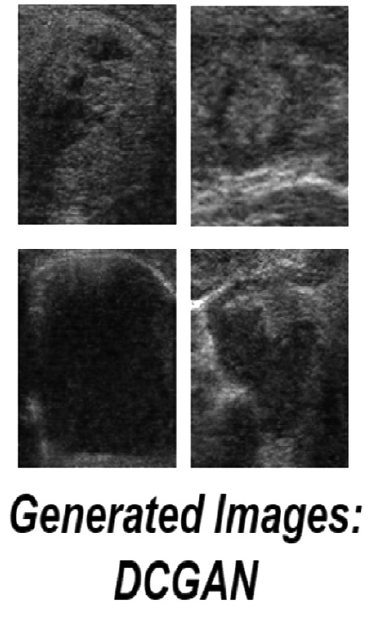
\includegraphics[width=0.35\textwidth]{2/figures/vitpaper6_part1.png}
		\caption[Imágenes de ultrasonido de la tiroides generadas]{Imágenes de ultrasonido de la tiroides generadas. \\
		Fuente: \cite{pr_JERBI2023autoclassViTGAN}. \textit{Automatic classification of ultrasound thyroids images using vision transformers and generative adversarial networks}.}
		\label{2:fig122}
	\end{center}
\end{figure}

La arquitectura del modelo generador consta de una entrada que es ruido generado aleatoriamente a través de una distribución normal estándar, luego se pasa a través de seis convoluciones 2D transpuestas (fractionally-strided convolution) con tamaño de kernel 4 x 4 con el fin de hacer up-sampling hasta llegar al tamaño de 128 x 128. Todas las capas convolucionales excepto la primera tienen un stride de 2. La primera tiene el stride definido en 1 pixel. Finalmente, se usa ReLU en todas las capas convolucionales a excepción del a última. 

La parte de la arquitectura encargada de discriminar tiene una entrada de tamaño 3 x 128 x 128. Este parte del modelo también incluye 6 capas de convolución 2D con un kernel de 4 x 4 y un stride de 2 para todas la capas a excepción de la capa final. Se usó Leaky ReLU con pendiente negativa de 0.2 como función de activación en todas la capas sin contar la capa final que se definió la función sigmoide.

Para la división del conjunto de datos, se usaron dos métodos distintos. El primero consistía en dividir el toda la data en 80\% para el entrenamiento (4 000 imágenes de nódulos benignos y 4 000 imágenes de nódulos malignos), 10\% (500 benignos y 500 malignos) para la validación y 10\% (500 benignos y 500 malignos) para la prueba. El segundo método fue el cross-validation con k-fold de tamaño de 10; es decir, se tomaron 9 000 imágenes para el entrenamiento y 1 000 para la prueba.

Las Redes Neuronales Convolucionales VGG16, EffecientNetB0 y ResNet50 se probaron con el conjunto de datos (dividido por los dos métodos mencionados) utilizando Transfer Learning. En la parte del clasificador se usó Softmax y SVM con un kernel igual a l2. Esta parte sirvió para definir cuál modelo CNN será usado para la implementación de la arquitectura híbrida.

La arquitectura de ViT usada fue el ViTB16. Este modelo recibe patches de 16 x 16. Es decir, las imágenes de ultrasonido se dividirán, de acuerdo a su tamaño, en patches de tamaño 16 x 16. Luego, cada uno de estos es aplanado y mapeado a través de una proyección lineal.

A la secuencia de embedded patches se le añade un nuevo tipo de embedding a la posición 0. Además, se añade otros embeddings 1D a cada embedded patch que indiquen sus respectivas posiciones. Esto finalmente será usado en el encoder del transformer.

El Transformer Encoder consta de un Multi-Head Self Attention (MSA) y un Perceptrón Multicapa (MLP) (dos capas con función GELU), donde la salida del MSA es alimentada al MLP.

La investigación propone que en lugar de alimentar con patches al modelo transformer, se use las salidas de un modelo CNN (ResNet50) como entrada. Esto se logra a través de pasar por un proceso de patching a los tensores resultantes del modelo CNN.

Los modelos CNN y ViT fueron entrenados con los mismos hiper-parámetros (optimizador SGD, tasa de aprendizaje de 0.0001, tamaño de lote de 32, 20 épocas e imágenes de 128 x 128).

En el caso específico de los modelos ViT se usó la función de activación Softmax con la función de pérdida Binary-Cross Entropy. En el caso del clasificador SVM, se usó el kernel l2, función de activación lineal y función de pérdida hinge.

Las métricas usadas para evaluar los modelos entrenados fueron el Accuracy, Precision, Recall y F1-score.

Los resultados se muestran en la Tabla \ref{2:table28}.

\begin{table}[H]
	\caption[Comparación de los modelos entrenados]{Comparación de los modelos entrenados.}
	\label{2:table28}
	\centering
	\small
	\begin{tabular}{ccccccc}
		\specialrule{.1em}{.05em}{.05em}
		{} & {Modelo} & {División de datos} & {F1-score} & {Recall} & {Precision} & {Accuracy} \\
		\specialrule{.1em}{.05em}{.05em}
		\multirow{10}{4cm}{Softmax Classifier} & {VGG16} & {División clásica} & {93.06\%} & {93.06\%} & {93.06\%} & {92.90\%} \\
		{} & {EffecientNetB0} & {División clásica} & {86.42\%} & {86.42\%} & {86.42\%} & {86.40\%} \\
		{} & {RestNet50} & {División clásica} & {96.67\%} & {96.67\%} & {96.67\%} & {96.60\%} \\
		{} & {ViT-B16} & {División clásica} & {92.28\%} & {92.28\%} & {92.28\%} & {92.10\%} \\
		{} & {Hybrid ViT} & {División clásica} & {97.87\%} & {97.87\%} & {97.87\%} & {97.50\%} \\

		{} & {VGG16} & {10-Folds} & {93.24\%} & {93.24\%} & {93.24\%} & {93.42\%} \\
		{} & {EffecientNetB0} & {10-Folds} & {87.09\%} & {87.09\%} & {87.09\%} & {87.16\%} \\
		{} & {RestNet50} & {10-Folds} & {96.66\%} & {96.66\%} & {96.66\%} & {96.71\%} \\
		{} & {ViT-B16} & {10-Folds} & {96.10\%} & {96.10\%} & {96.10\%} & {95.98\%} \\
		{} & {Hybrid ViT} & {10-Folds} & {96.96\%} & {96.96\%} & {96.96\%} & {97.10\%} \\

		\multirow{10}{4cm}{SVM Classifier} & {VGG16} & {División clásica} & {92.78\%} & {90.82\%} & {94.96\%} & {93.69\%} \\
		{} & {EffecientNetB0} & {División clásica} & {85.38\%} & {76.85\%} & {96.42\%} & {90.79\%} \\
		{} & {RestNet50} & {División clásica} & {95.98\%} & {94.14\%} & {98.03\%} & {97.20} \\
		{} & {ViT-B16} & {División clásica} & {94.55\%} & {92.08\%} & {97.23\%} & {95.09\%} \\
		{} & {Hybrid ViT} & {División clásica} & {96.42\%} & {94.82\%} & {98.24\%} & {96.80\%} \\

		{} & {VGG16} & {10-Folds} & {92.29\%} & {90.86\%} & {93.98\%} & {93.44\%} \\
		{} & {EffecientNetB0} & {10-Folds} & {83.95\%} & {75.38\%} & {95.46\%} & {90.51\%} \\
		{} & {RestNet50} & {10-Folds} & {96.46\%} & {94.96\%} & {98.16\%} & {97.32\%} \\
		{} & {ViT-B16} & {10-Folds} & {96.12\%} & {95.14\%} & {97.18\%} & {96.17\%} \\
		{} & {Hybrid ViT} & {10-Folds} & {96.67\%} & {95.01\%} & {98.51\%} & {97.63\%} \\

		\specialrule{.1em}{.05em}{.05em}
	\end{tabular}
	\begin{flushleft}	
		\small Fuente: \cite{pr_JERBI2023autoclassViTGAN}. \textit{Automatic classification of ultrasound thyroids images using vision transformers and generative adversarial networks}.
	\end{flushleft}
\end{table}

En relación a los modelos CNN, se pudo observar que el de mayor desempeño fue el RestNet50 con el clasificador SVM, alcanzando un accuracy de 97.32\%. Este hallazgo permitió determinar el CNN a usar en el modelo híbrido propuesto (ResNet50-ViTB16) que obtuvo finalmente el mejor desempeño general con un accuracy de 97.63\%.

Según \cite{pr_gong2022ACL} encontrar un nódulo tiroideo es relativamente común en varios casos clínicos, pues tiene una tasa de incidencia del 19\% al 68\%, de los cuales un 5\% al 15\% son malignos. Además, existe una gran variedad de imágenes médicas que puede pueden ser usadas para su diagnóstico, siendo las imágenes de ultrasonido la de mayor uso al momento de diagnósticas si un nódulo tiroideo es benigno o maligno. Sin embargo, este tipo de imágenes tiene un gran problema, es que no existe un estándar definido para tomar este tipo de imágenes a diferencia de otros tipos de imágenes como lo son las imágenes tomográficas. Esto conlleva a que las imágenes de ultrasonido sean muy variantes, de distintas resoluciones y con diferentes niveles de ruido. Es por todo esto que se menciona la alta necesidad de desarrollar un siste CAD capaz de aumentar la precisión en el proceso de diagóstico de nódulo tiroideos.

Para el desarrollo de este tipo de sistema, en la investigación se propuso el uso de un nuevo marco de trabajo denominado Adaptative Curriculum Learning (ACL), utilizado en el proceso de entrenamiento y que es capaz de abordar el problema de etiquetas inconsistentes presente en la tarea de clasificación de nódulos tiroideos.

El framework ACL tiene la capacidad de forzar al modelo entrenado a enfocarse en primera instancia en las imágenes más fácilas de clasificar y, posteriormente, en las más difíciles de forma gradual. Aquellas imágenes con etiquetas inconsistentes son descartadas del proceso de entrenamiento otorgándoles una pérdida de cero.

En el proceso de entrenamiento, con cada mini lote de imágenes, el modelo realiza predicciones y el nivel de confianza sobre cada una de las muestras. Luego, en la cola de muestras difíciles, se añaden aquellas muestras que el modelo clasificó de forma incorrecta, mientras que en la cola de certeza, se añaden las confianzas máximas calculadas de cada predicción realizada en el lote. Ya con estas dos colas pobladas, se procede a calcular el umbral adaptativo (T-ada) a través de ambas colas. Este umbral es usado para determinar la forma de cálculo de las pérdidas: si la confianza de predicción es superior al umbral, se calcula la pérdida a través de la entropía cruzada, en caso contrario, la muestra es descartada y se le asigna una pérdida de cero. Finalmente, la pérdida total del lote es calculada a través de la suma de todas las pérdidas de aquellas muestras que no han sido descartadas. Esta pérdida total calculada es usada para el proceso de retropropagación del modelo.

Todo este proceso de entrenamiento con el ACL se puede observar en la Figura \ref{2:fig123}.

\begin{figure}[H]
	\begin{center}
		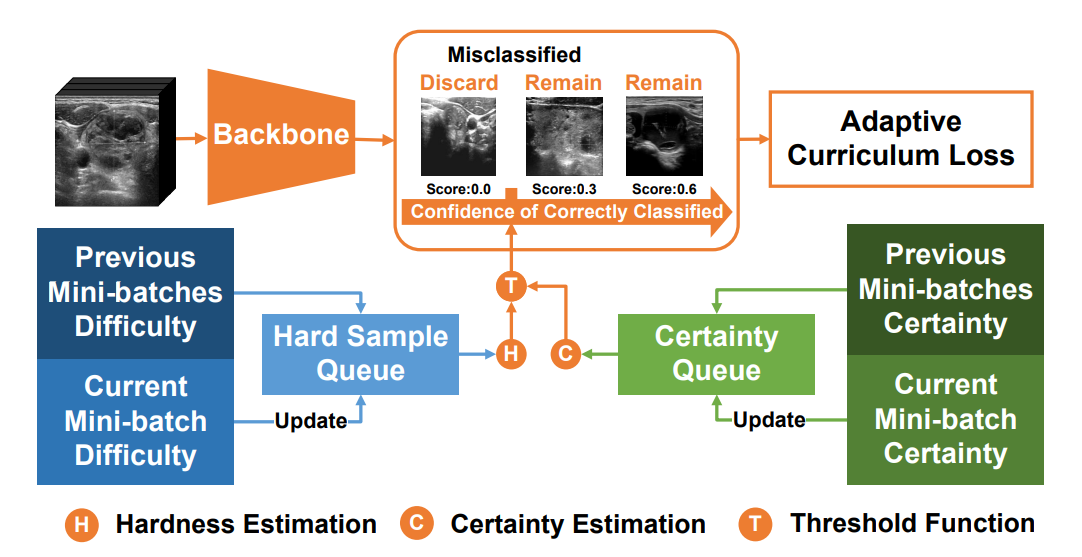
\includegraphics[width=0.80\textwidth]{2/figures/acl_process.png}
		\caption[Proceso de entrenamiento con ACL]{Proceso de entrenamiento con ACL. \\
		Fuente: \cite{pr_gong2022ACL}. \textit{Less is More: Adaptive Curriculum Learning for Thyroid Nodule Diagnosis}.}
		\label{2:fig123}
	\end{center}
\end{figure}

Para realizar el entrenamiento de sus modelos con ACL, en la investigación se propone el uso del conjunto de datos TNCD (Thyroid Nodule Classification Dataset) que consiste de 3 493 imágenes de ultrasonido de nódulos tiroideos de 2 421 pacientes, y dividido en subconjuntos de entrenamiento y prueba, con el primero que consta de 2 879 imágenes (1 905 benignos y 974 malignos) y el segundo de 614 imágenes (378 benignos y 236 malignos). Este conjunto de datos es otorgado por el mismo repositorio online y de acceso libre de los investigadores, con el fin de facilitar futuras investigaciones en el área.

Los backbone utilizados para el proceso de entrenamiento junto con el ACL fueron las arquitecturas de ResNet18, DenseNet121 y ConvNeXt-Tiny. Estos modelos fueron comparados con otras funciones de pérdida basadas en el aprendizaje curricular avanzado (Curriculum Loss y SuperLoss) y aplicadas con los mismos backbone.

Todos los modelos fueron entrenados con el NVIDIA 3090 GPU y Pytorch. Los pesos iniciales fueron fueron sacados de las arquitecturas preentrenadas con ImageNet. El optimizador fue el Stochastic Gradient Descent (SGD) y una tasa de aprendizaje de 0.001. Las imágenes fueron redimensionadas a 224 x 224 píxeles, y se aplicó un aumento a través de un giro horizontal. Este proceso de Aumento de datos se aplicó a la clase minoritaria (imágenes de nódulos benignos). Finalmente, se definió a 16 el tamaño de lote y cantidad de épocas.

Los resultados del entrenamiento se presentan en la Tabla \ref{2:table29}.

\begin{table}[H]
	\caption[Resultados del entrenamiento de los modelos con ACL]{Resultados del entrenamiento de los modelos con ACL.}
	\label{2:table29}
	\centering
	\small
	\begin{tabular}{p{2.8cm}cccccc}
		\specialrule{.1em}{.05em}{.05em}
		{Est. de Aprendizaje} & {Backbone} & {Accuracy} & {Precision} & {Recall} & {F1-score} & {AUC} \\
		\specialrule{.1em}{.05em}{.05em}
		\multirow{3}{4cm}{Cross Entropy} & {ResNet18} & {70.75\%} & {61.71\%} & {68.05\%} & {64.47\%} & {77.31\%} \\
		{} & {DenseNet121} & {70.36\%} & {63.92\%} & {63.31\%} & {63.31\%} & {78.05\%} \\
		{} & {ConvNeXt-Tiny} & {72.29\%} & {62.94\%} & {71.19\%} & {66.36\%} & {78.38\%} \\
		\hline
		\multirow{3}{4cm}{CL} & {ResNet18} & {70.54\%} & {62.87\%} & {65.85\%} & {64.04\%} & {76.98\%} \\
		{} & {DenseNet121} & {70.03\%} & {62.44\%} & {65.25\%} & {63.31\%} & {77.27\%} \\
		{} & {ConvNeXt-Tiny} & {72.14\%} & {60.21\%} & {75.76\%} & {67.00\%} & {74.37\%} \\
		\hline
		\multirow{3}{4cm}{SL} & {ResNet18} & {71.26\%} & {64.97\%} & {64.15\%} & {64.46\%} & {78.50\%} \\
		{} & {DenseNet121} & {71.82\%} & {64.38\%} & {66.86\%} & {65.42\%} & {78.98\%} \\
		{} & {ConvNeXt-Tiny} & {71.47\%} & {62.66\%} & {68.39\%} & {65.36\%} & {77.87\%} \\
		\hline
		\multirow{3}{4cm}{ACL} & {ResNet18} & {73.28\%} & {63.02\%} & {73.64\%} & {67.87\%} & {79.89\%} \\
		{} & {DenseNet121} & {72.92\%} & {60.74\%} & {77.80\%} & {67.99\%} & {79.84\%} \\
		{} & {ConvNeXt-Tiny} & {72.50\%} & {61.19\%} & {74.75\%} & {67.21\%} & {78.85\%} \\
		\specialrule{.1em}{.05em}{.05em}
	\end{tabular}
	\begin{flushleft}	
		\small Fuente: \cite{pr_gong2022ACL}. \textit{Less is More: Adaptive Curriculum Learning for Thyroid Nodule Diagnosis}.
	\end{flushleft}
\end{table}

Los resultados muestran la superioridad de la estrategia de aprendizaje con ACL en comparación con las otras estrategias de aprendizaje, superando en las métricas de Accuracy, F1-score y AUC a los demás modelos.